\section{Additional CR Data and MC Comparisons} 
\label{app:ttdlnj}

This appendix shows some additional comparisons of the data and MC background samples
for various CRs. Figure~\ref{fig:cr1lepptdphi} shows some
additional components of the \mt, the lepton \pt\ and the
azimuthal angle between the lepton and the \met\ for CR1
(Section~\ref{sec:cr1}). Figure~\ref{fig:cr2lepptdphi} shows the
equivalent distributions for CR2 (Section~\ref{sec:cr2}), the positive lepton \pt\ and the
angle between this lepton and the
pseudo-\met. Similarly, figure~\ref{fig:cr5lepptdphi100} shows the lepton
\pt\ and and the azimuthal angle between the lepton and the \met\ for CR5
(Section~\ref{sec:cr5}). Figures~\ref{fig:cr4lepptdphi100}
and~\ref{fig:cr4dphidR100} provide some data and MC comparisons of the
\ttdl\ control sample CR4 (Section~\ref{sec:cr4}) for various
kinematic distributions: leading lepton \pt\ and eta, as well as the
angles between the two leptons and between the leading lepton and the
\met. These distributions show quite good agreement between data and
MC. More quantitative information is included in the section discussing each
control region.

\begin{figure}[hbt]
  \begin{center}
        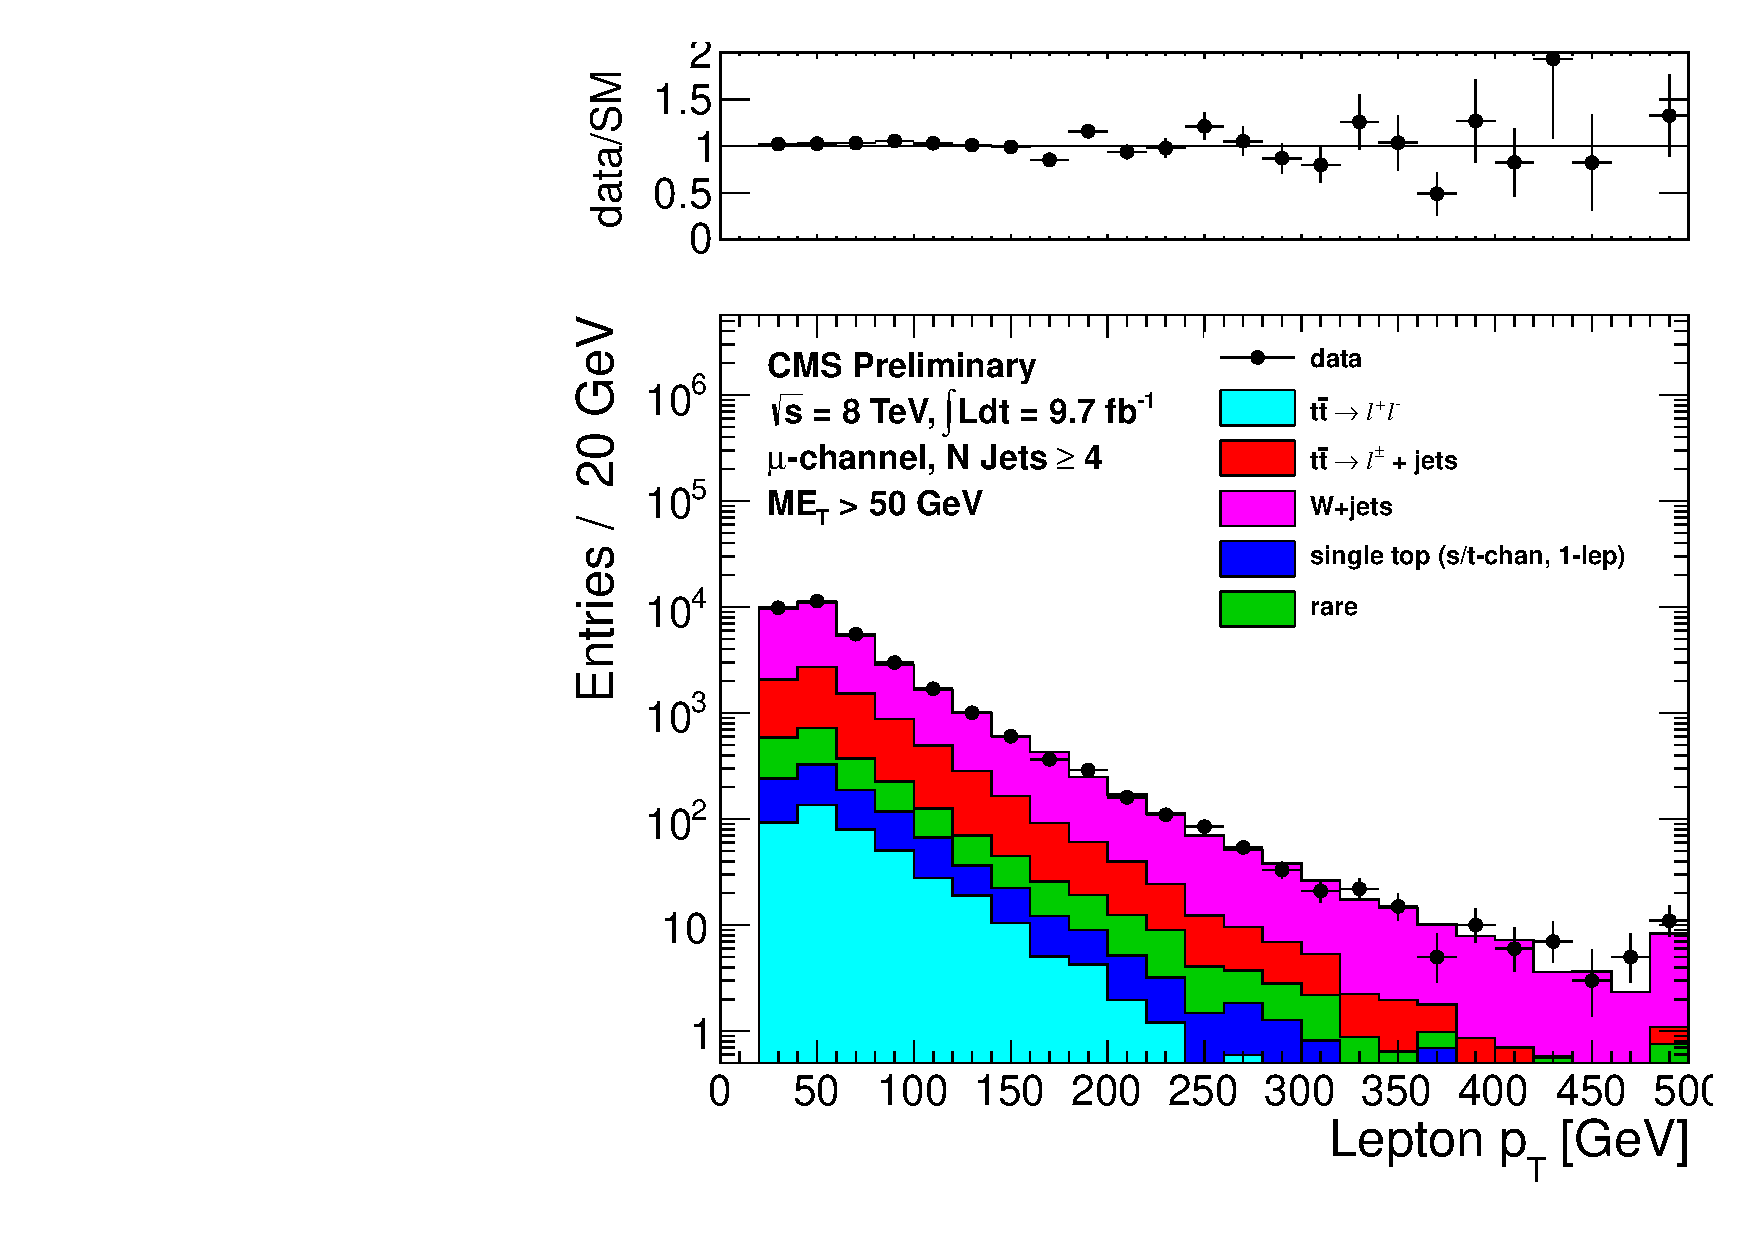
\includegraphics[width=0.5\linewidth]{plots/CR1plots/leppt_met50_leadmuo_nj4.pdf}%
        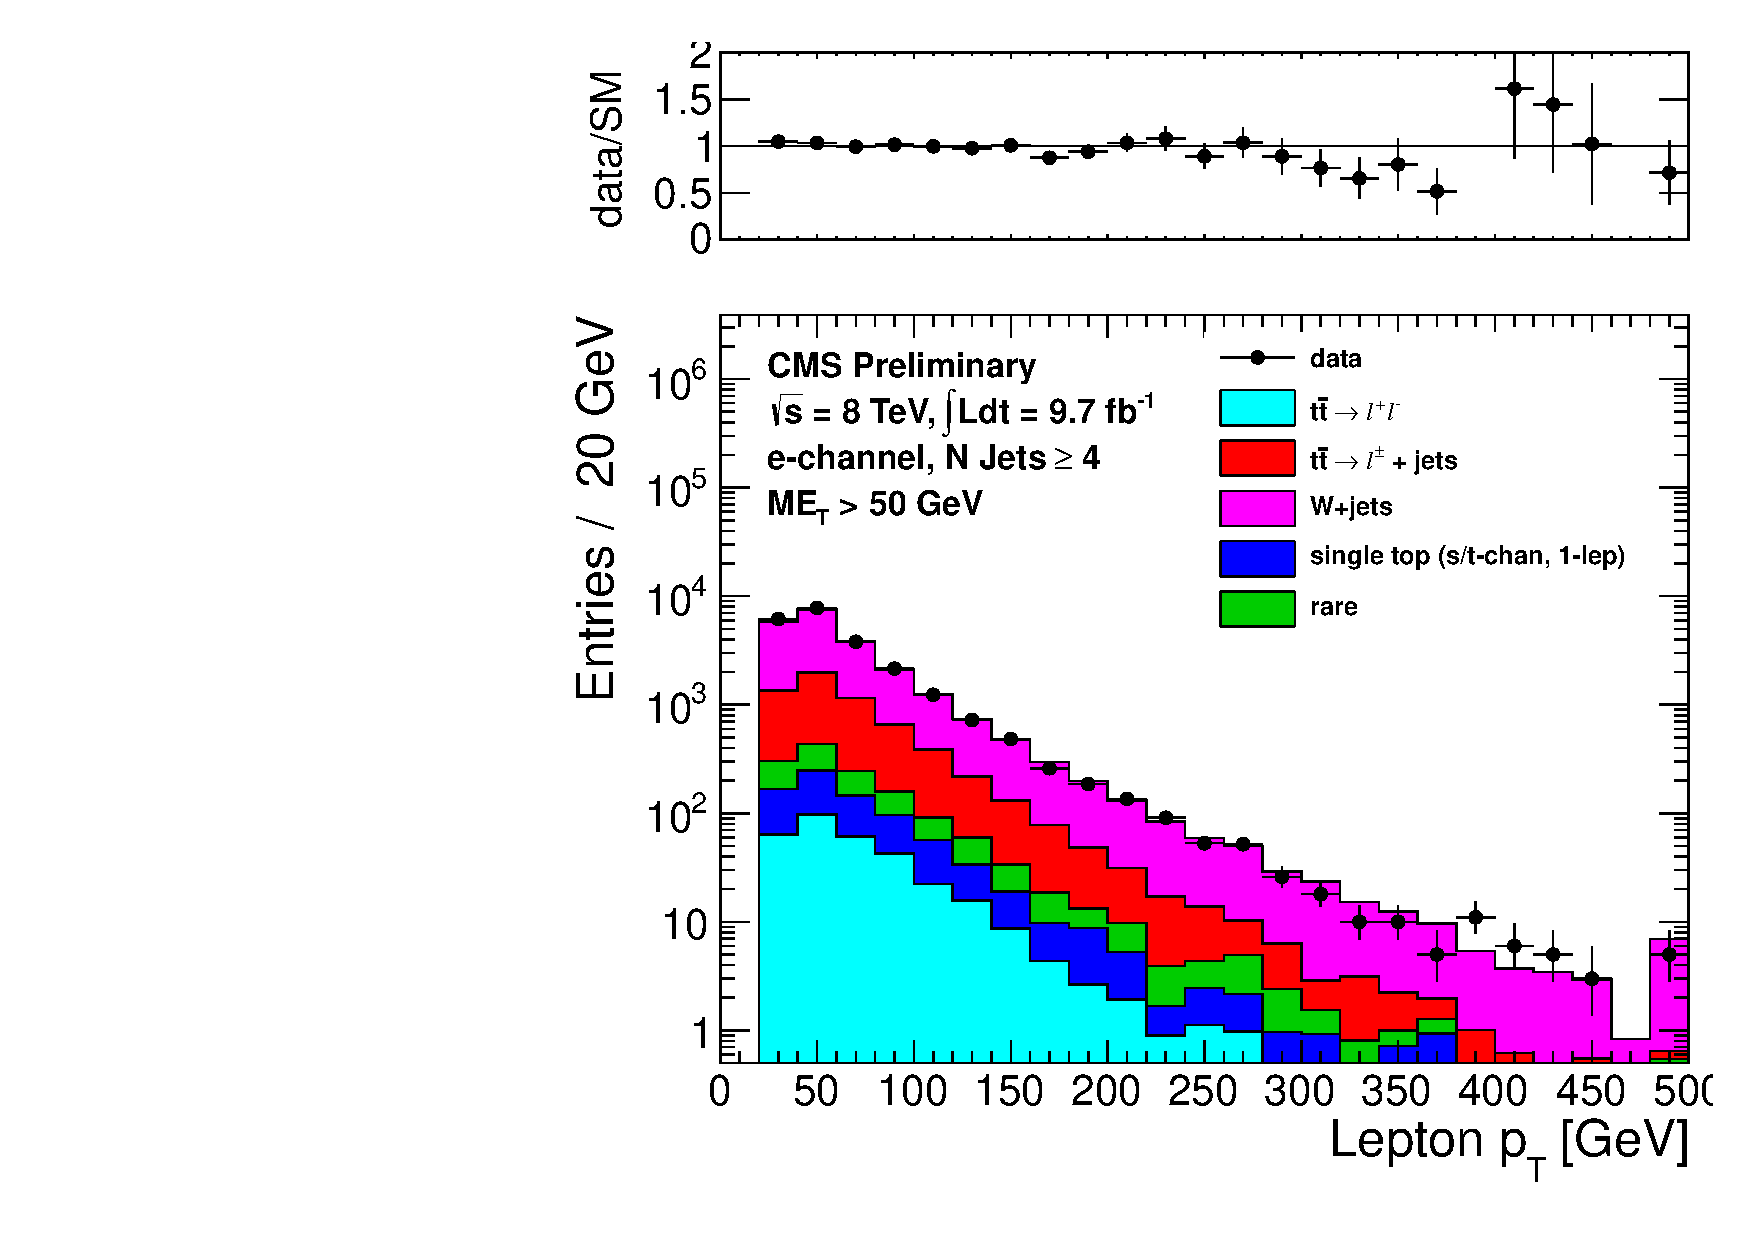
\includegraphics[width=0.5\linewidth]{plots/CR1plots/leppt_met50_leadele_nj4.pdf}
        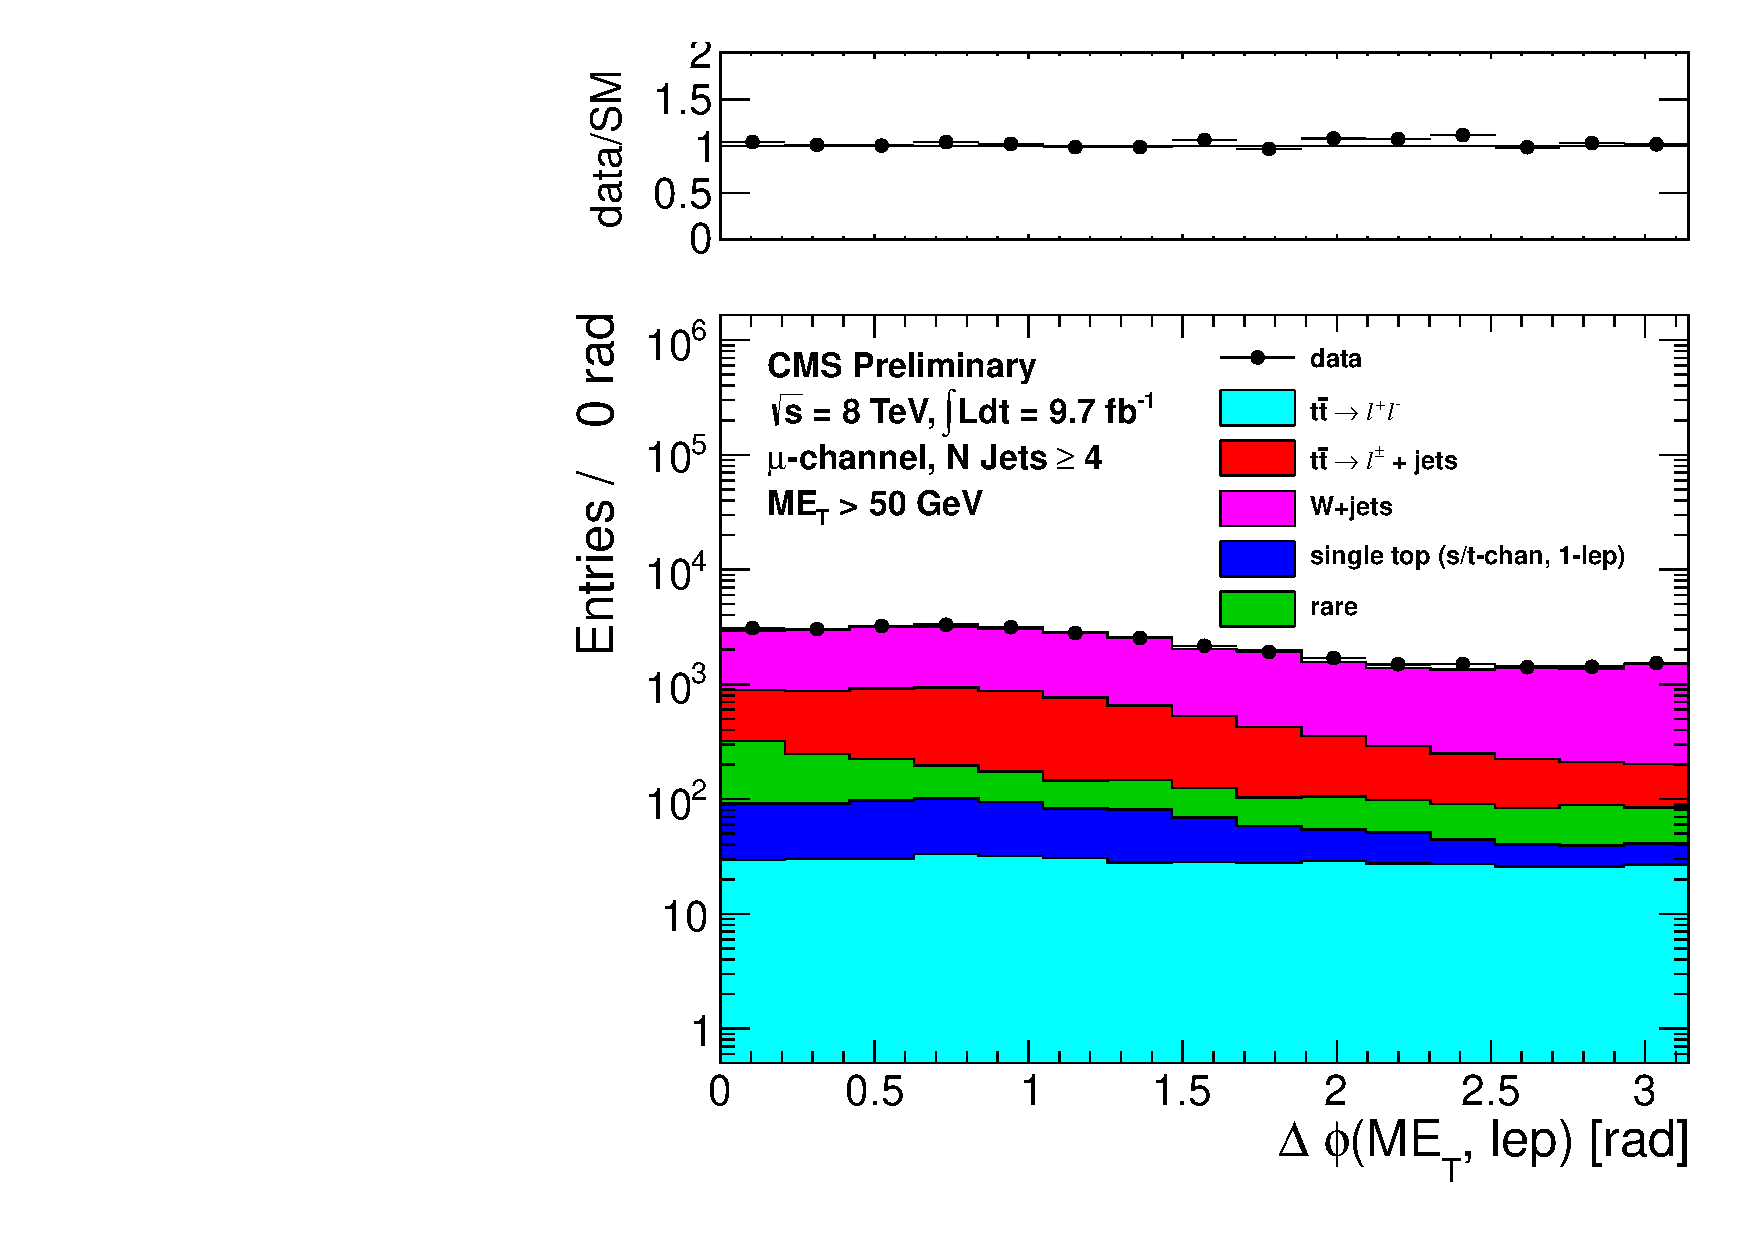
\includegraphics[width=0.5\linewidth]{plots/CR1plots/dphi_metlep_met50_leadmuo_nj4.pdf}%
        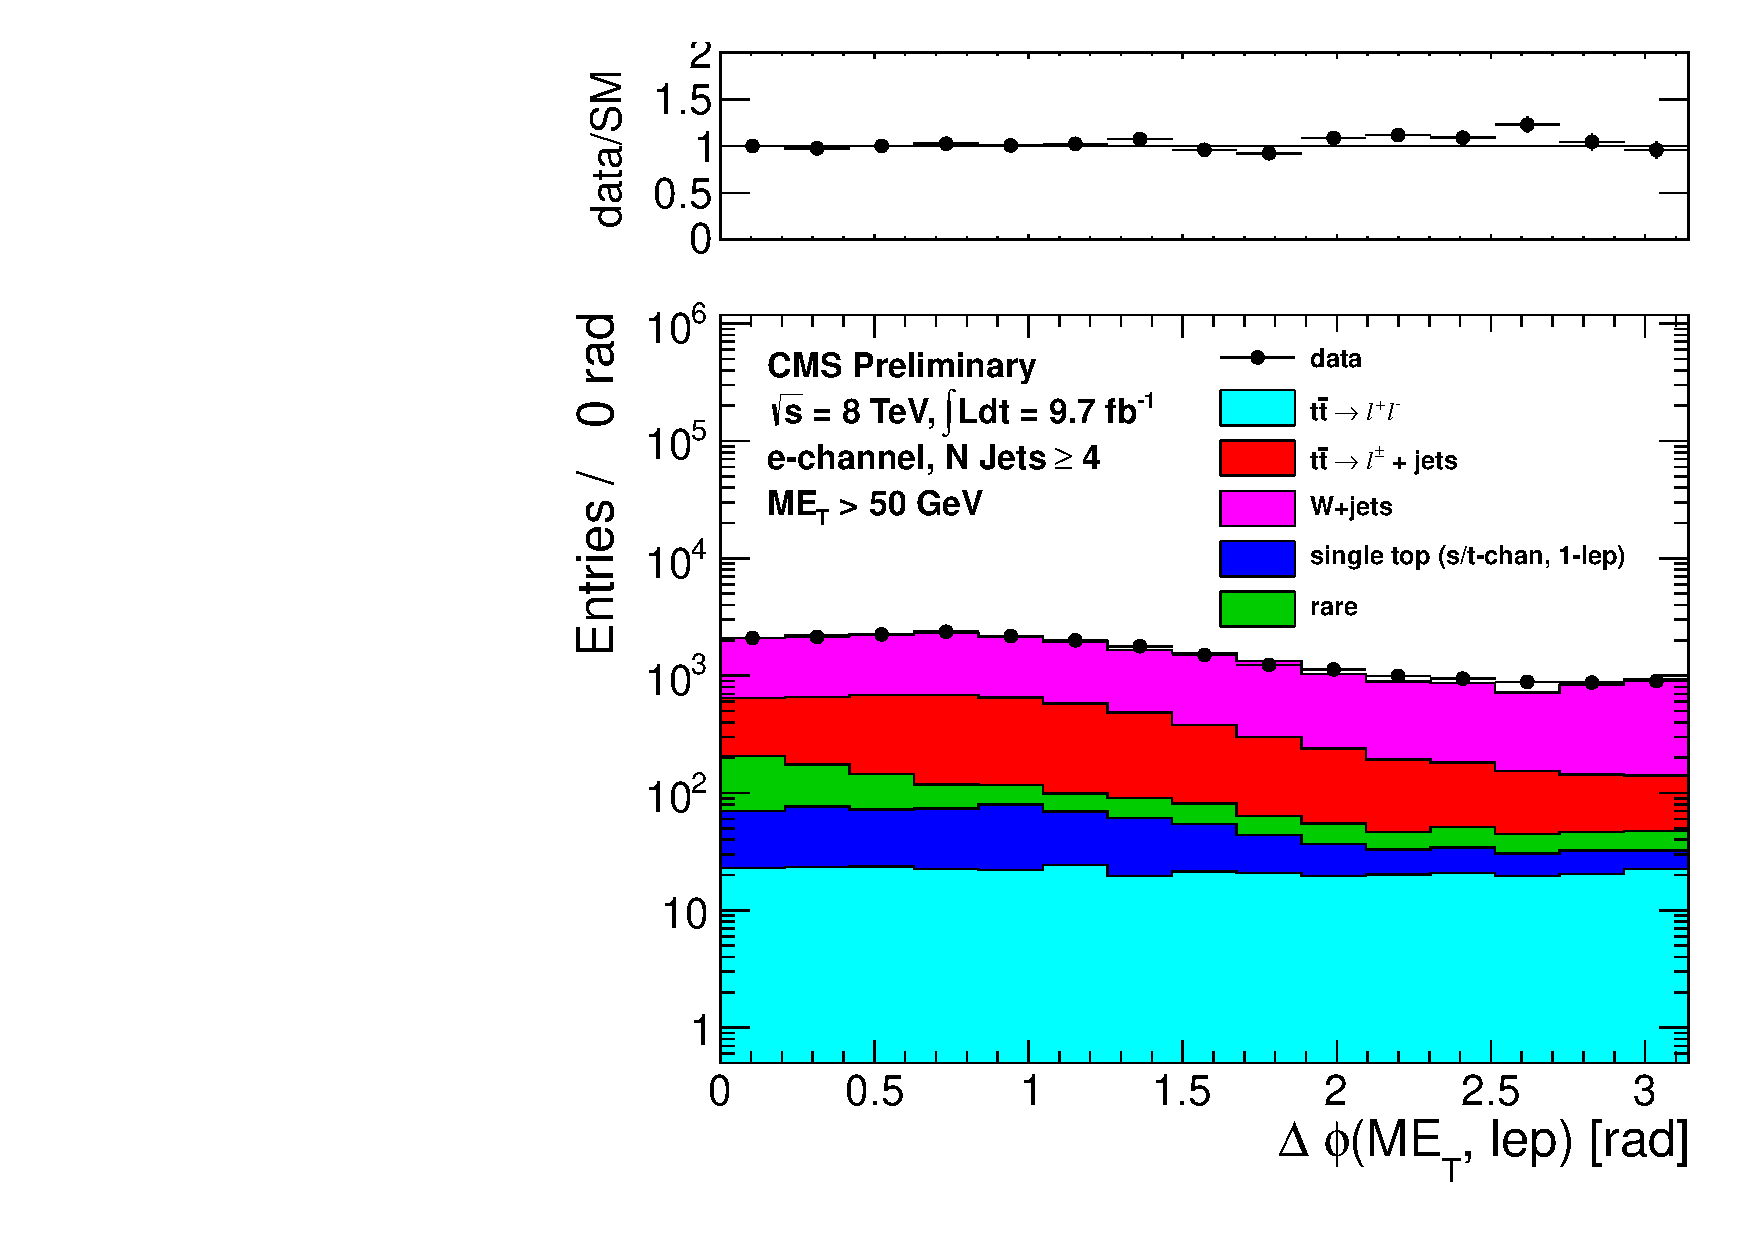
\includegraphics[width=0.5\linewidth]{plots/CR1plots/dphi_metlep_met50_leadele_nj4.pdf}
    \caption{
      Comparison of the lepton \pt\ (top) and azimuthal angle between the \met\ and the lepton (bottom) for 
      data vs. MC for events with a leading muon (left) and leading electron (right)
      satisfying the requirements of CR1. 
\label{fig:cr1lepptdphi} 
}  
      \end{center}
\end{figure}

\begin{figure}[hbt]
  \begin{center}
%	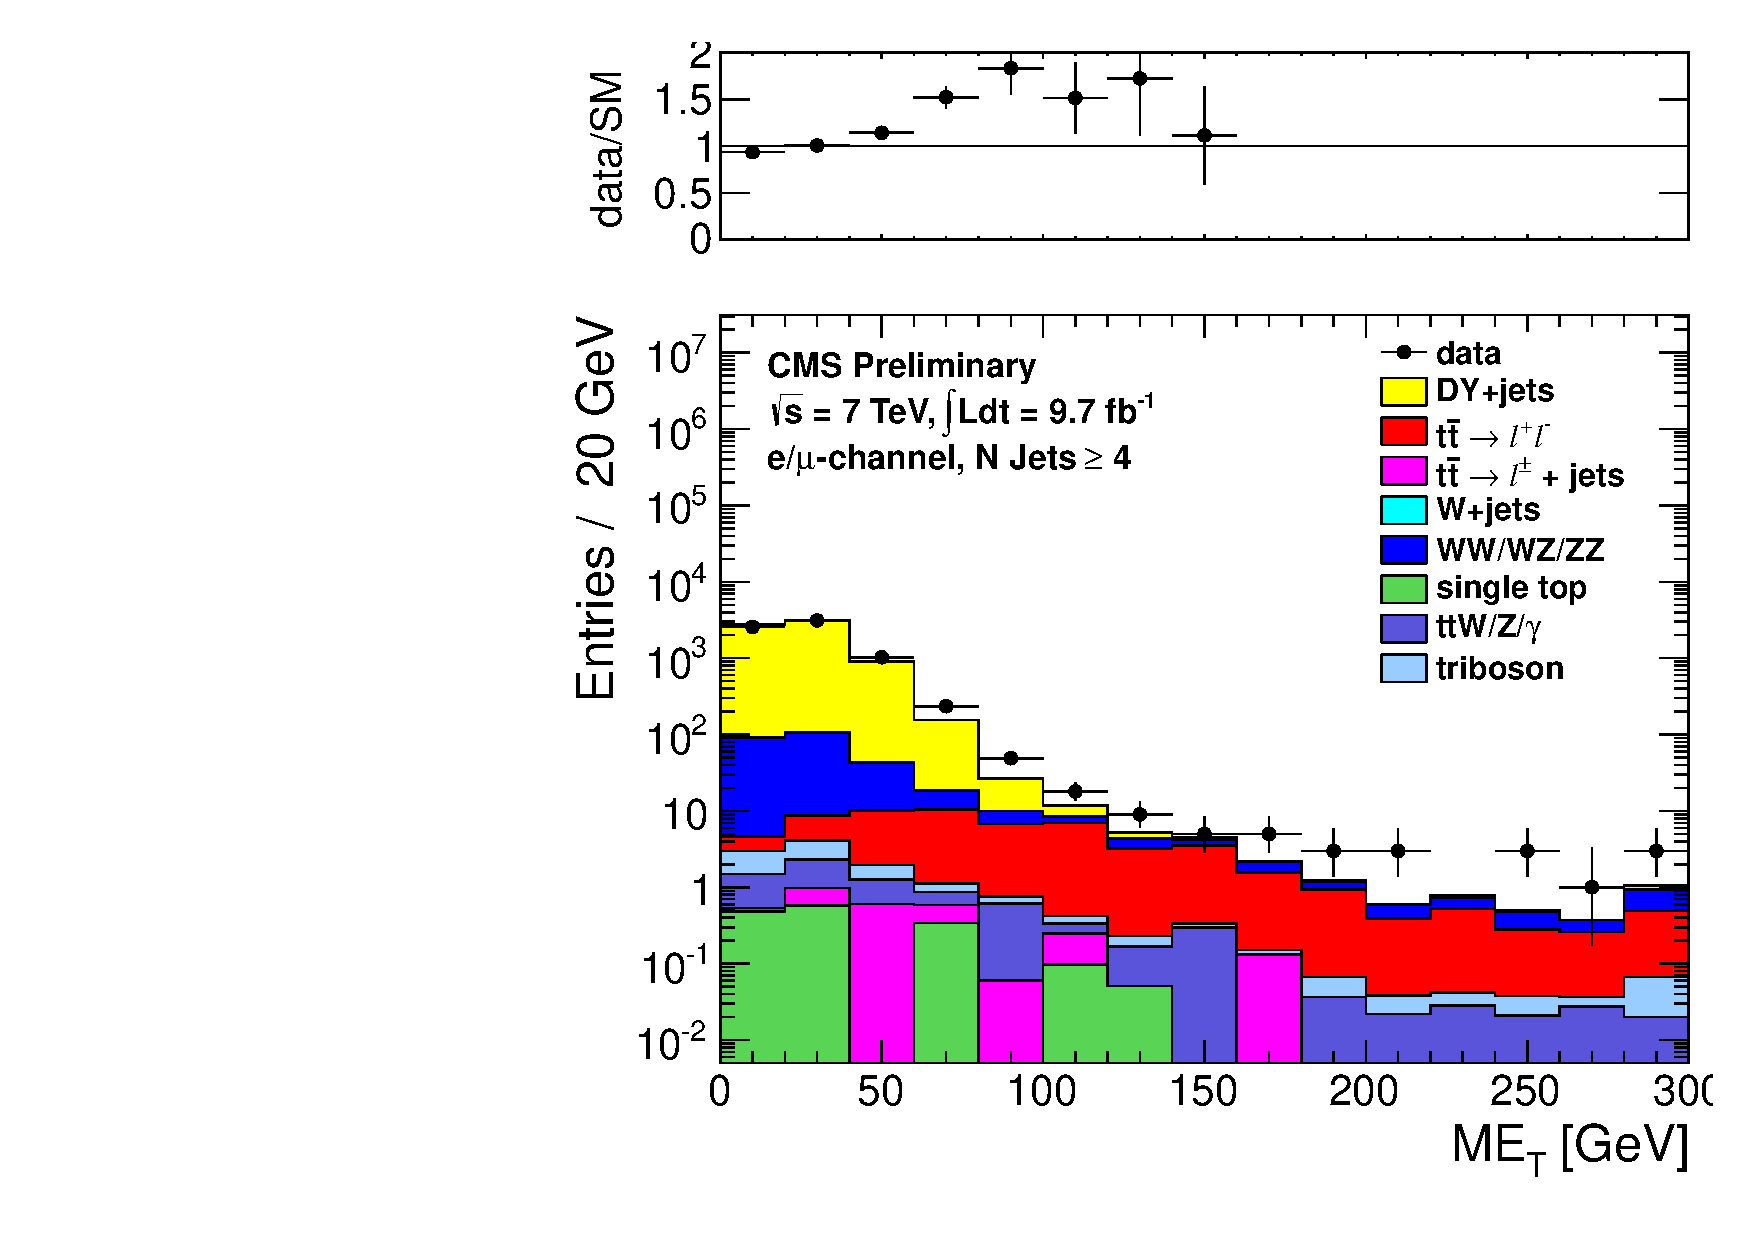
\includegraphics[width=0.5\linewidth]{plots/CR2plots/met_scaled_nj4_emucomb.pdf}%
	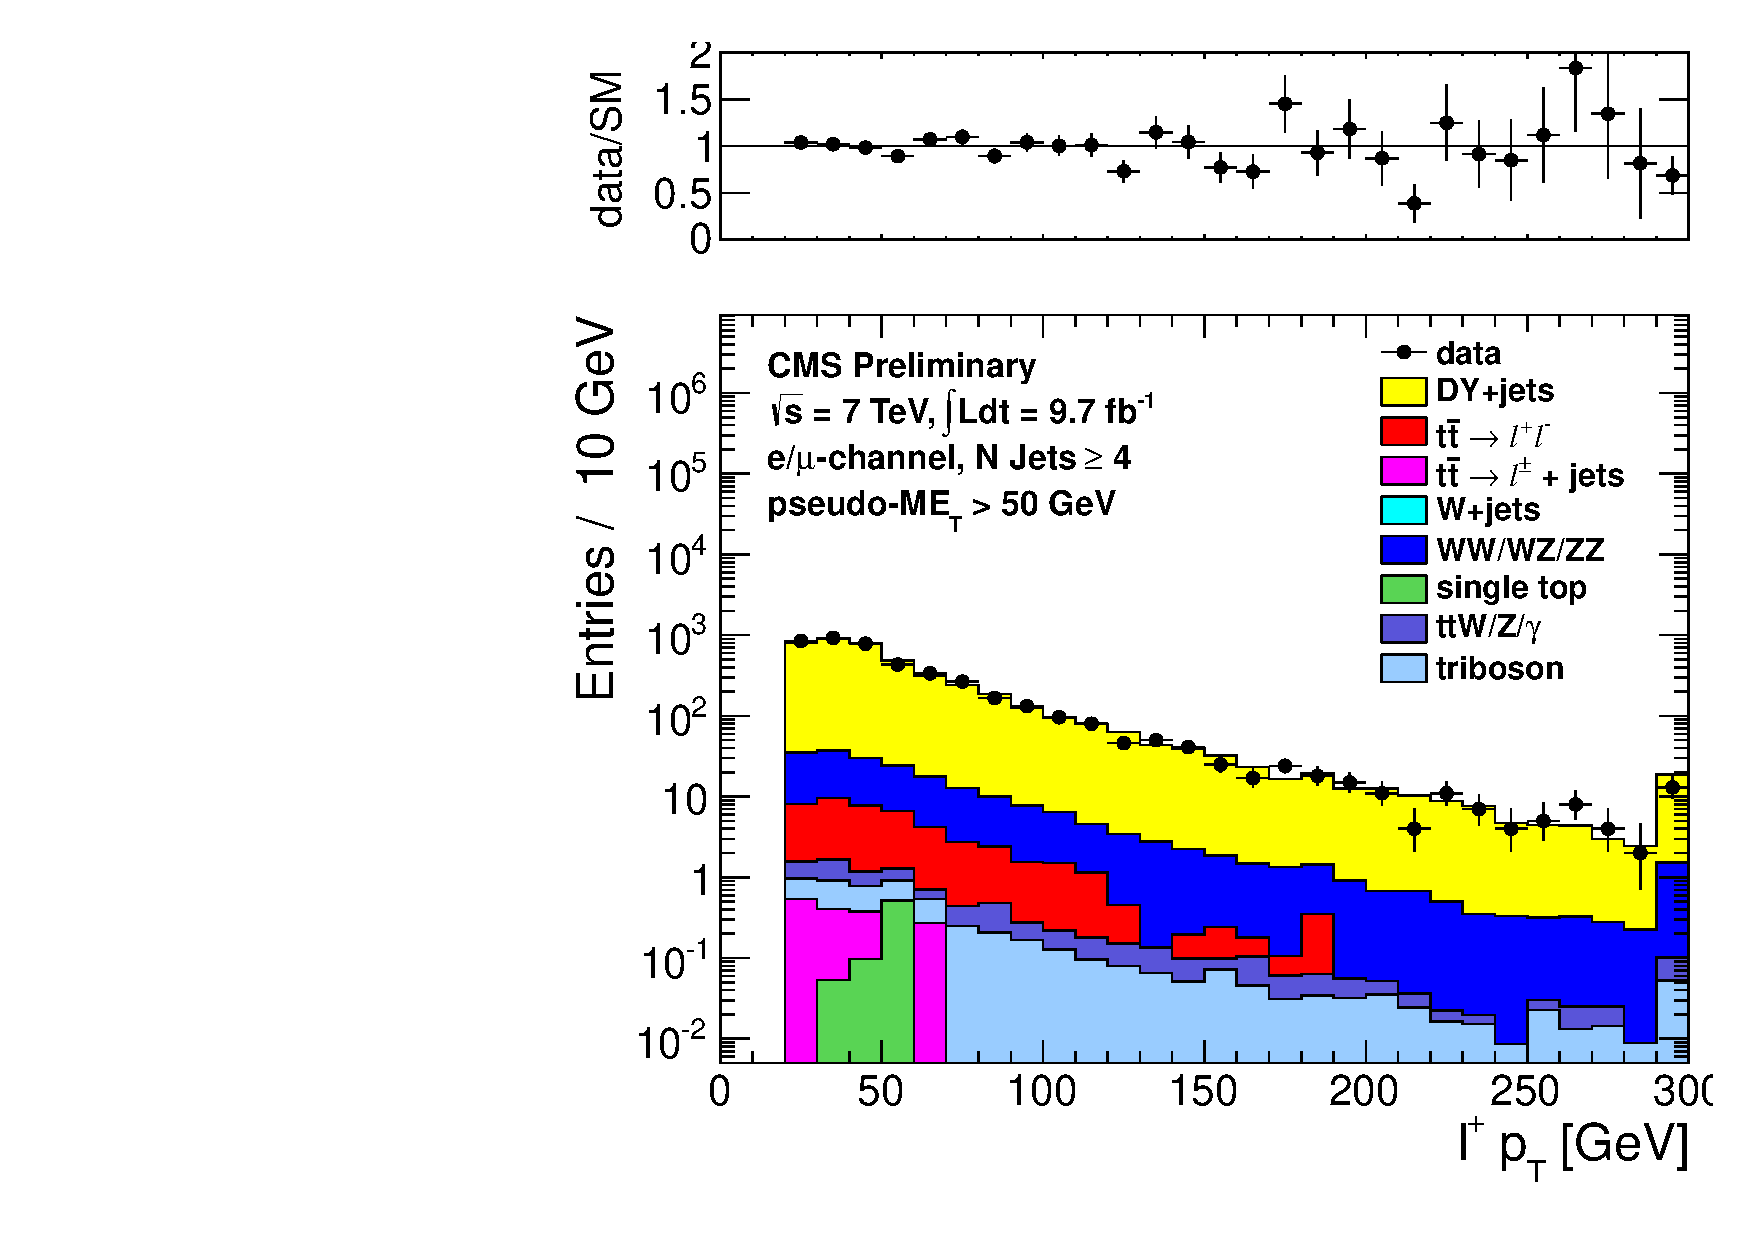
\includegraphics[width=0.5\linewidth]{plots/CR2plots/leppt_scaled_met50_nj4_emucomb.pdf}%
	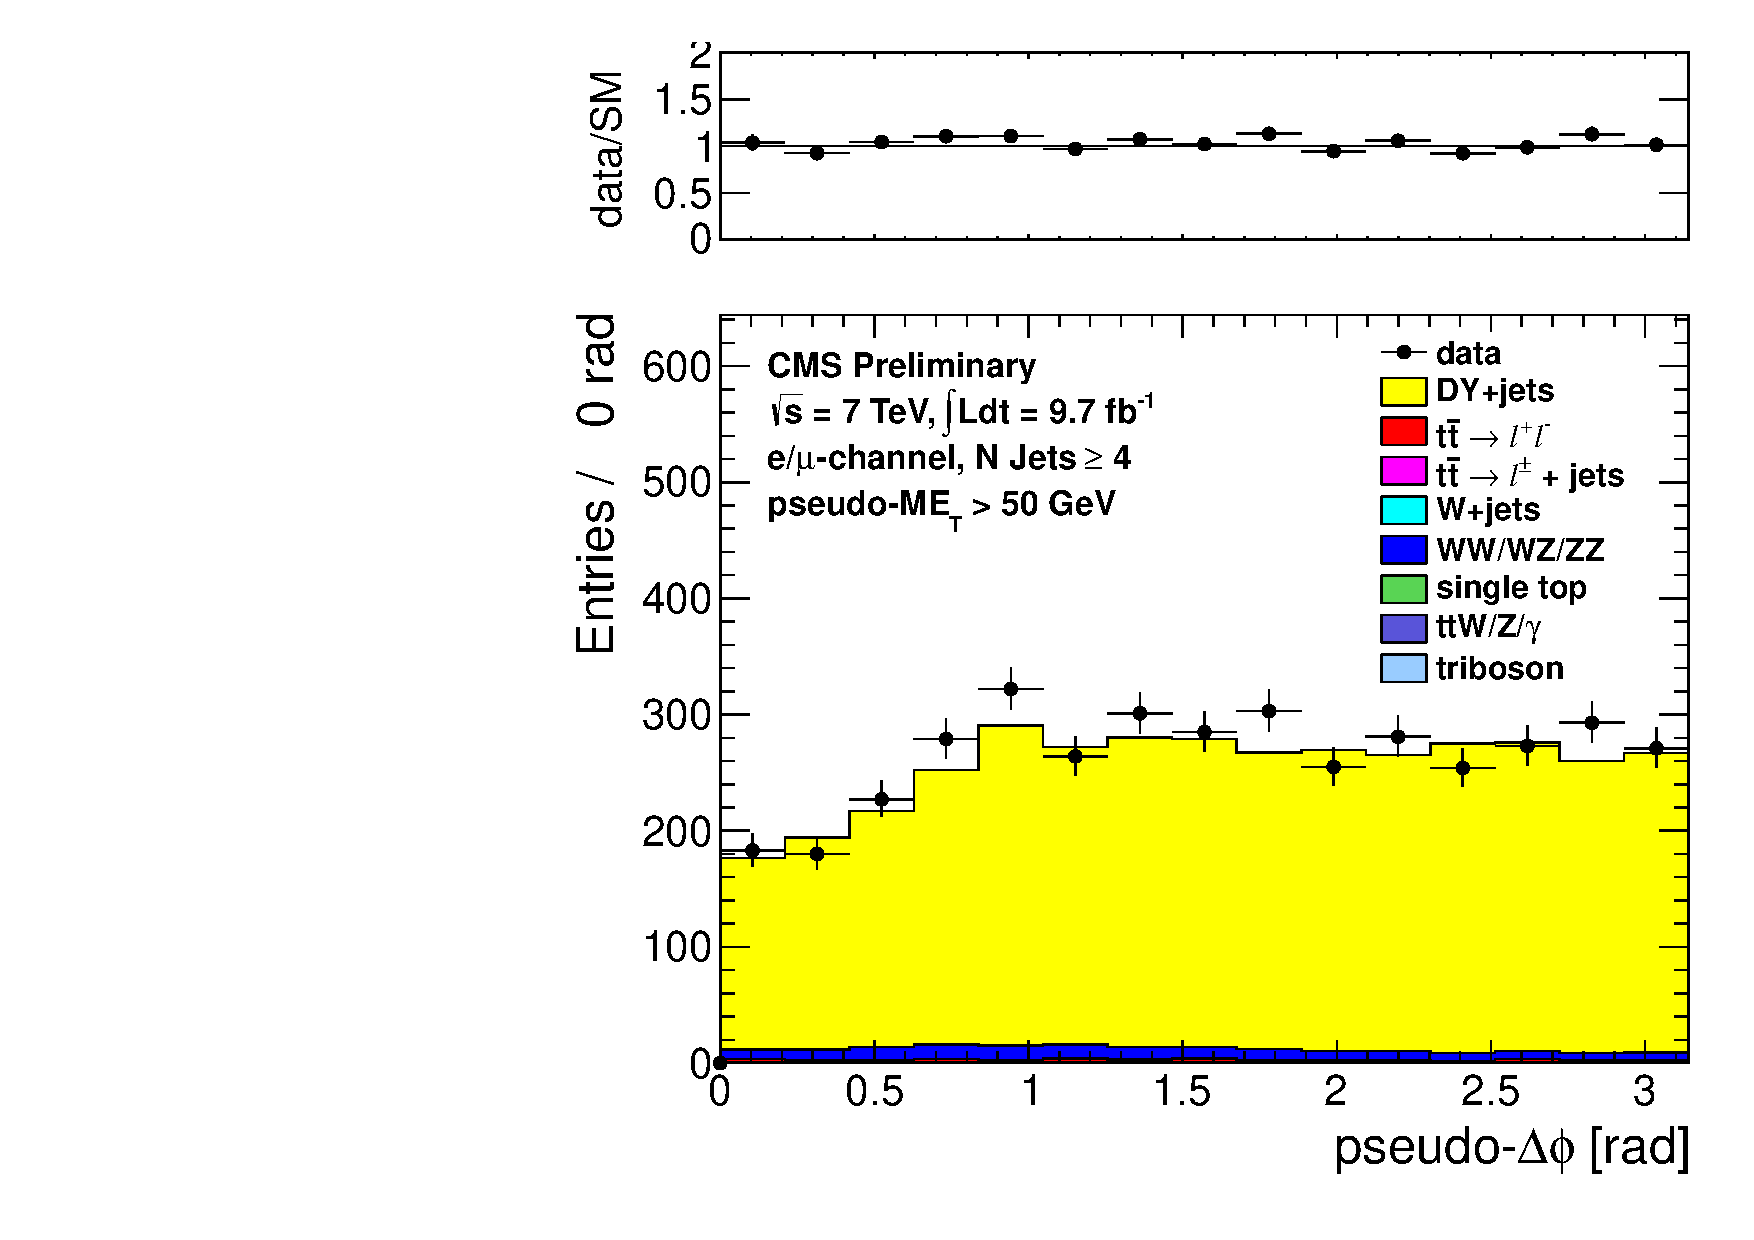
\includegraphics[width=0.5\linewidth]{plots/CR2plots/dphi_metl_scaled_met50_nj4_emucomb.pdf}
    \caption{
      Comparison of the positive lepton \pt\ (left) and the azimuthal angle between this lepton and the pseudo-\met\ (right) 
      distributions in data vs. MC for events satisfying the requirements of CR2, combining both the muon and
      electron channels. 
\label{fig:cr2lepptdphi} 
}  
      \end{center}
\end{figure}


\begin{figure}[hbt]
  \begin{center}
        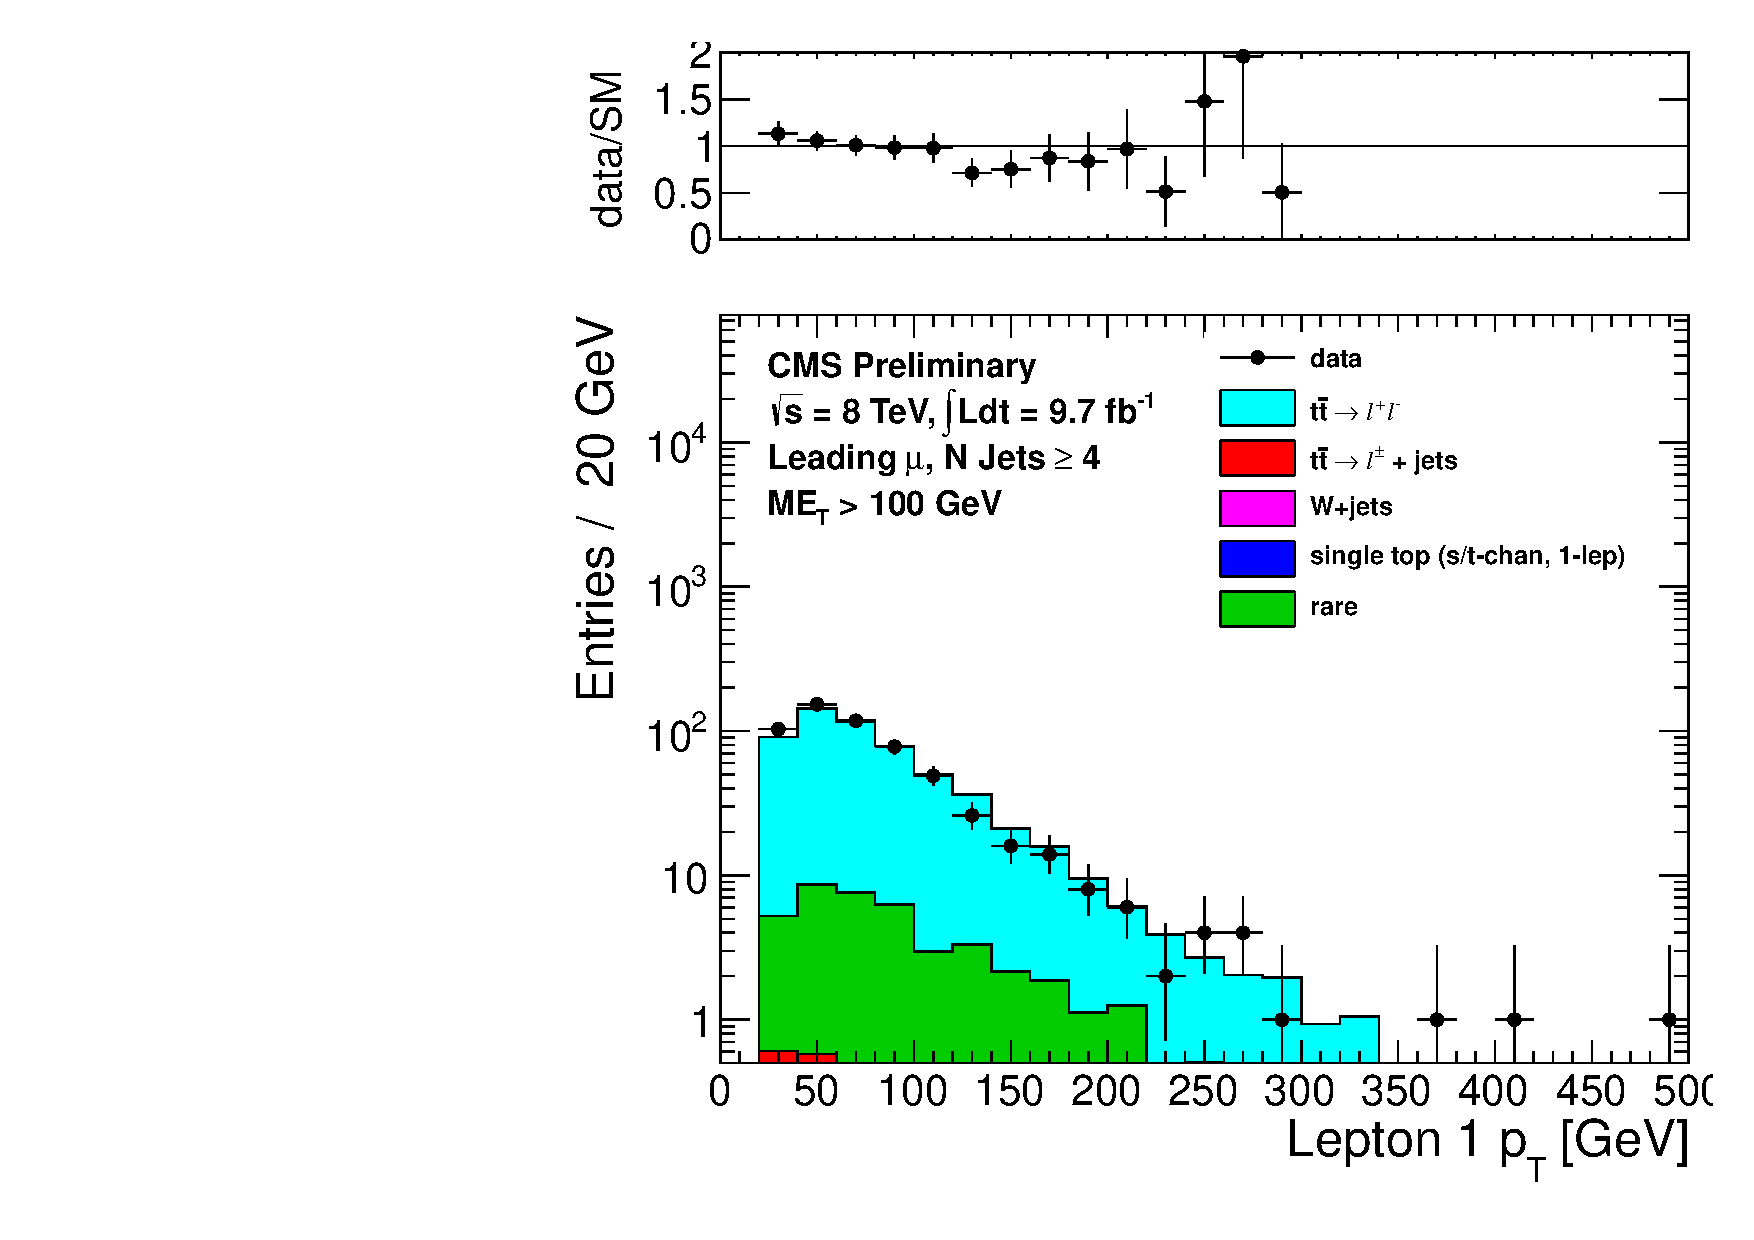
\includegraphics[width=0.5\linewidth]{plots/CR4plots/leppt_met100_leadmuo_nj4.pdf}%
        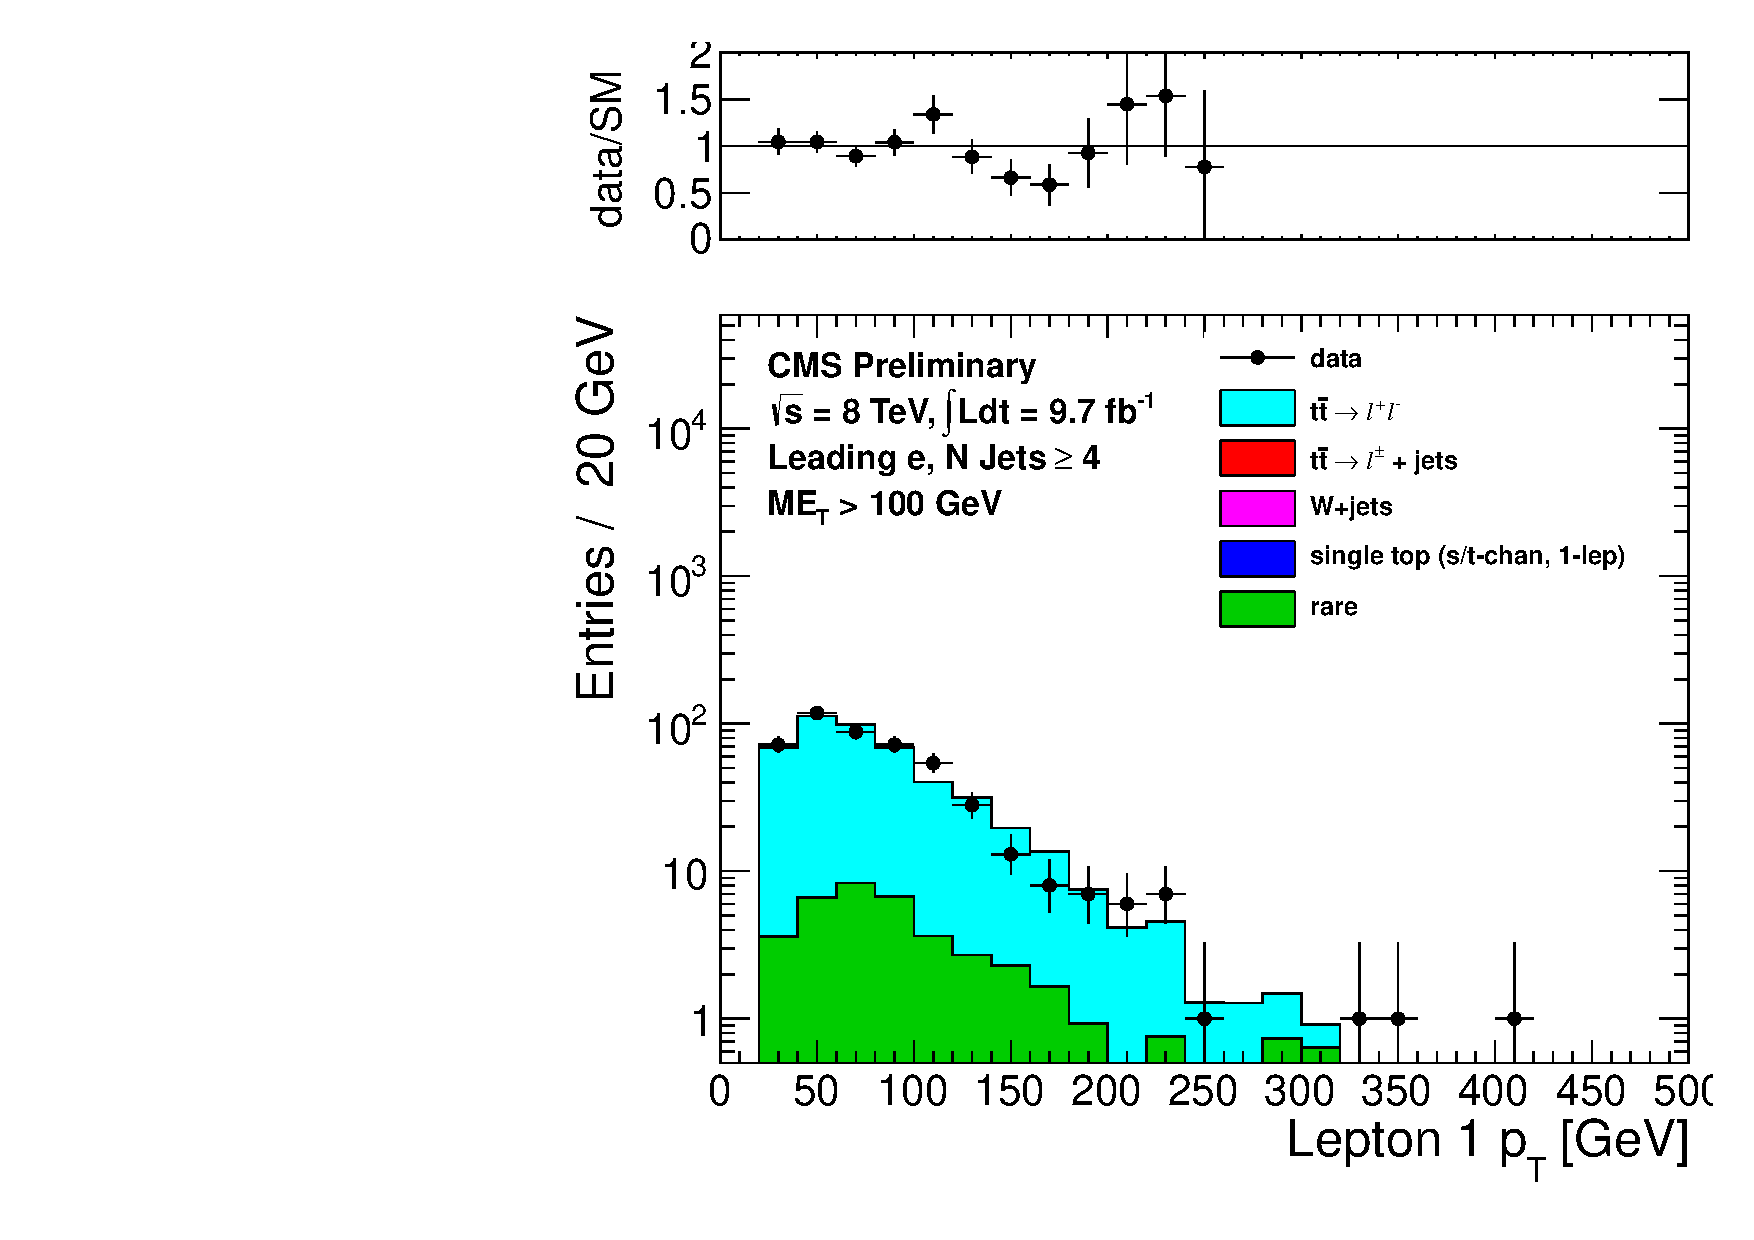
\includegraphics[width=0.5\linewidth]{plots/CR4plots/leppt_met100_leadele_nj4.pdf}
        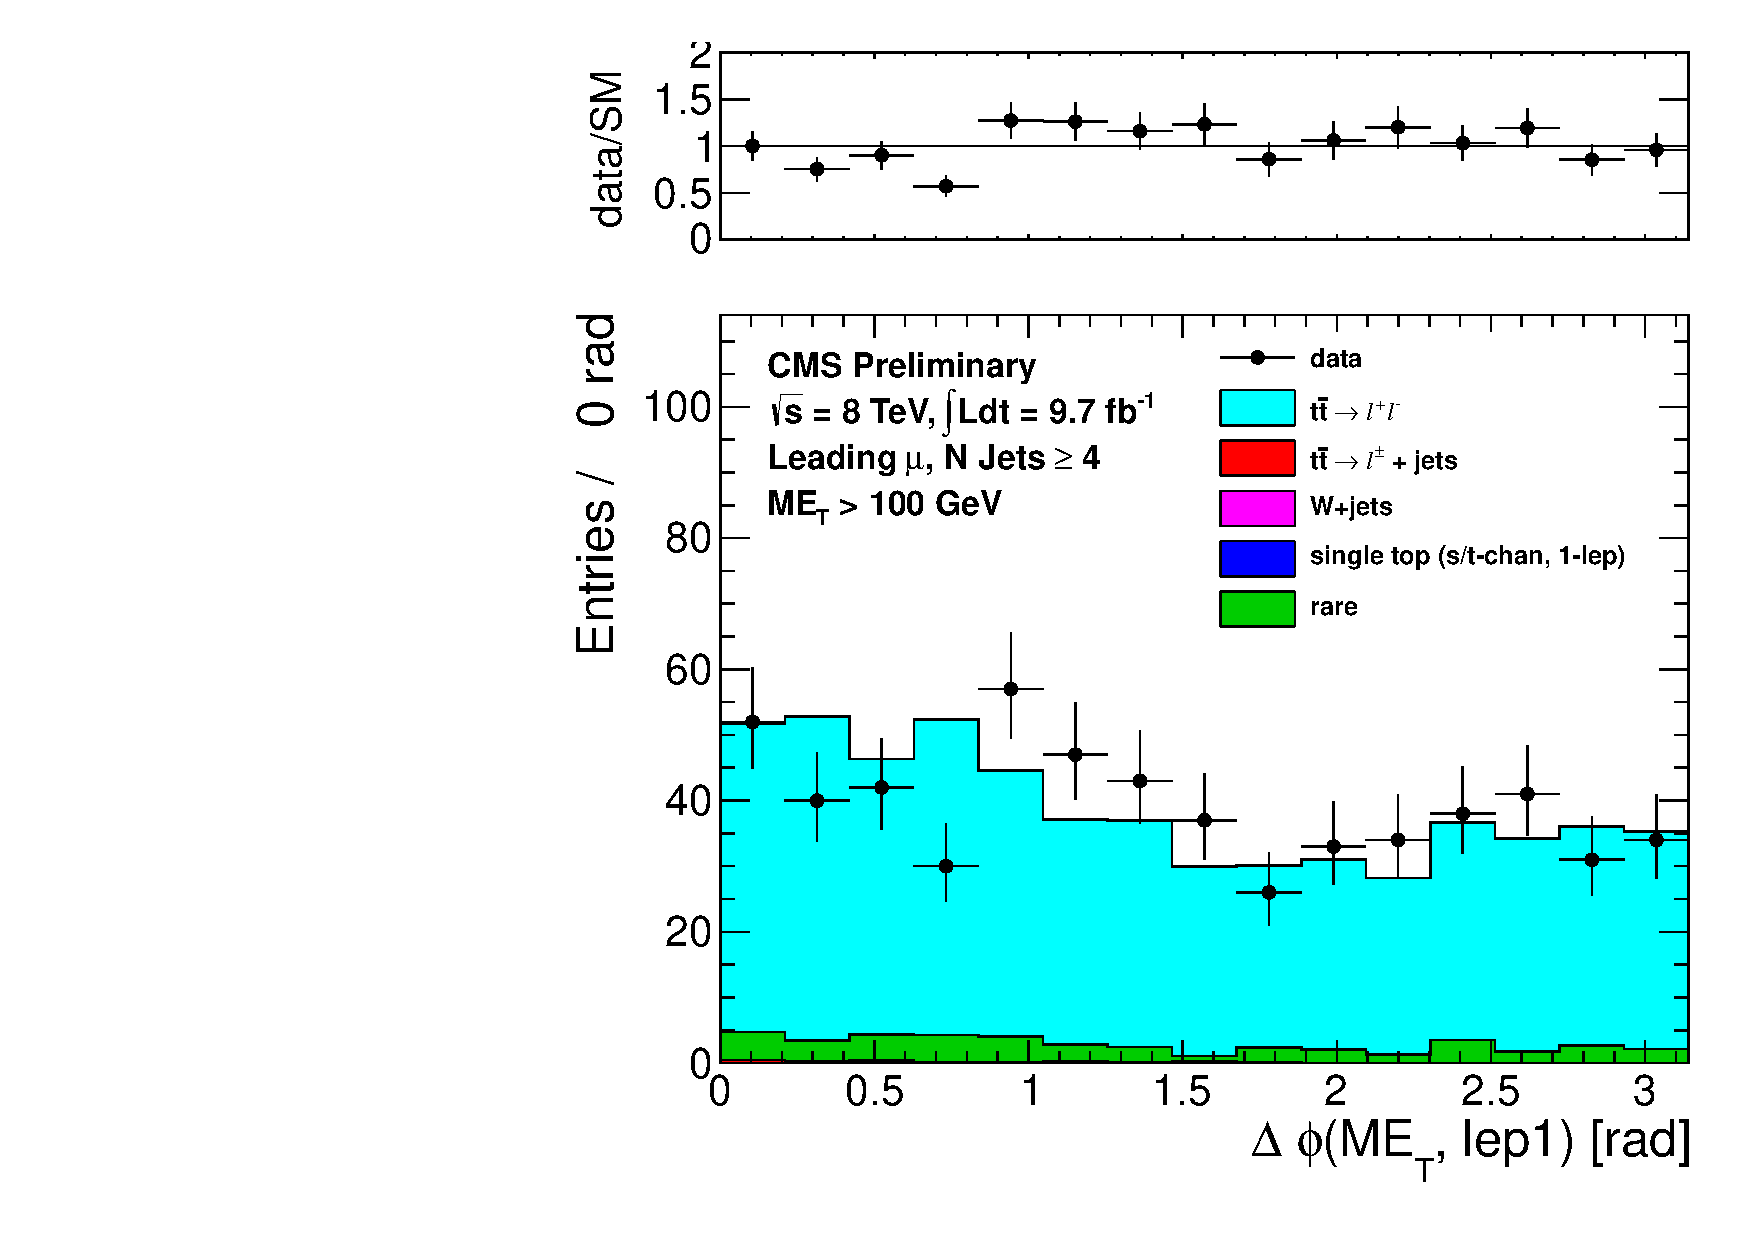
\includegraphics[width=0.5\linewidth]{plots/CR4plots/dphi_metlep_met100_leadmuo_nj4.pdf}%
        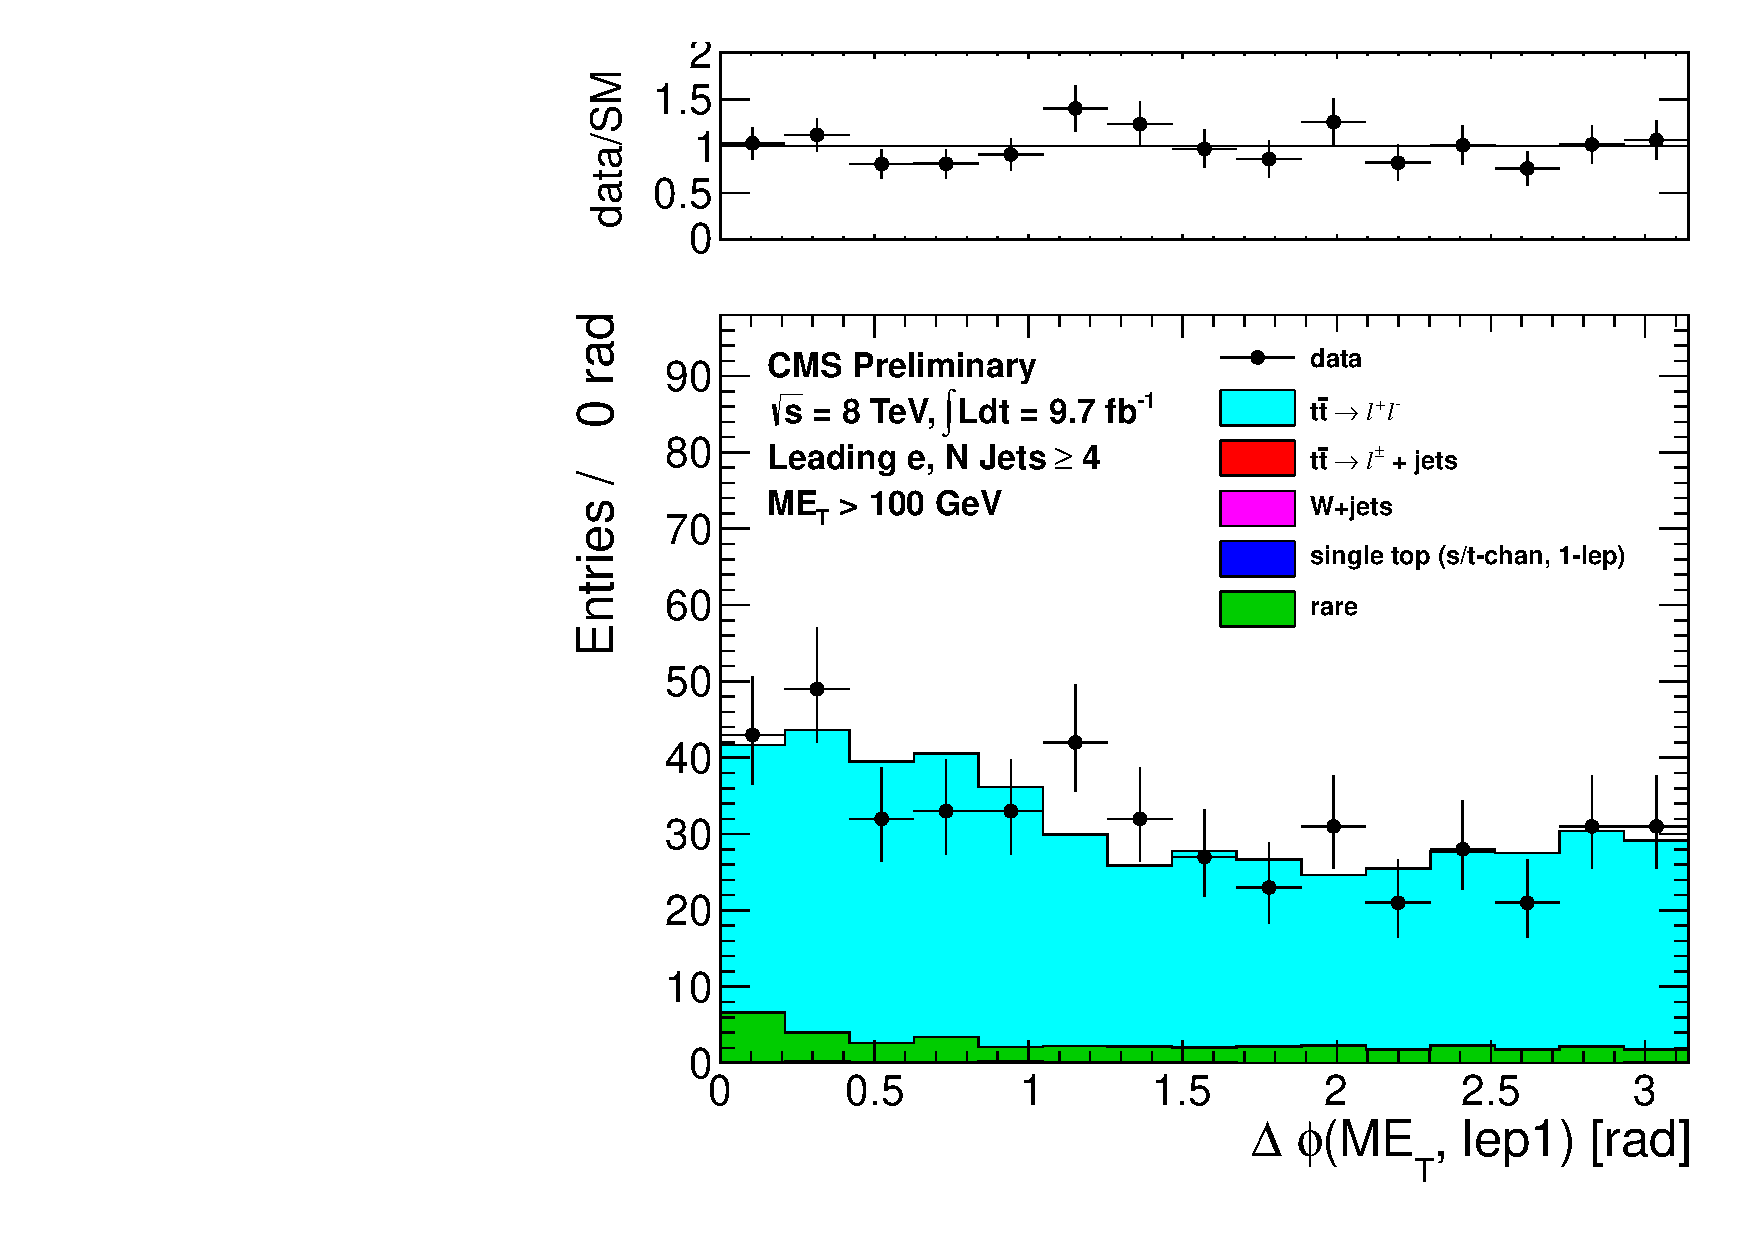
\includegraphics[width=0.5\linewidth]{plots/CR4plots/dphi_metlep_met100_leadele_nj4.pdf}
    \caption{
      Comparison of the leading lepton \pt\ (top) and azimuthal angle between the leading lepton and the \met\ 
      for $\met>100$ GeV distributions in data vs. MC for events
      with a leading muon (left) and leading electron (right)
      satisfying the requirements of CR4. 
\label{fig:cr4lepptdphi100} 
}  
      \end{center}
\end{figure}

\begin{figure}[hbt]
  \begin{center}
        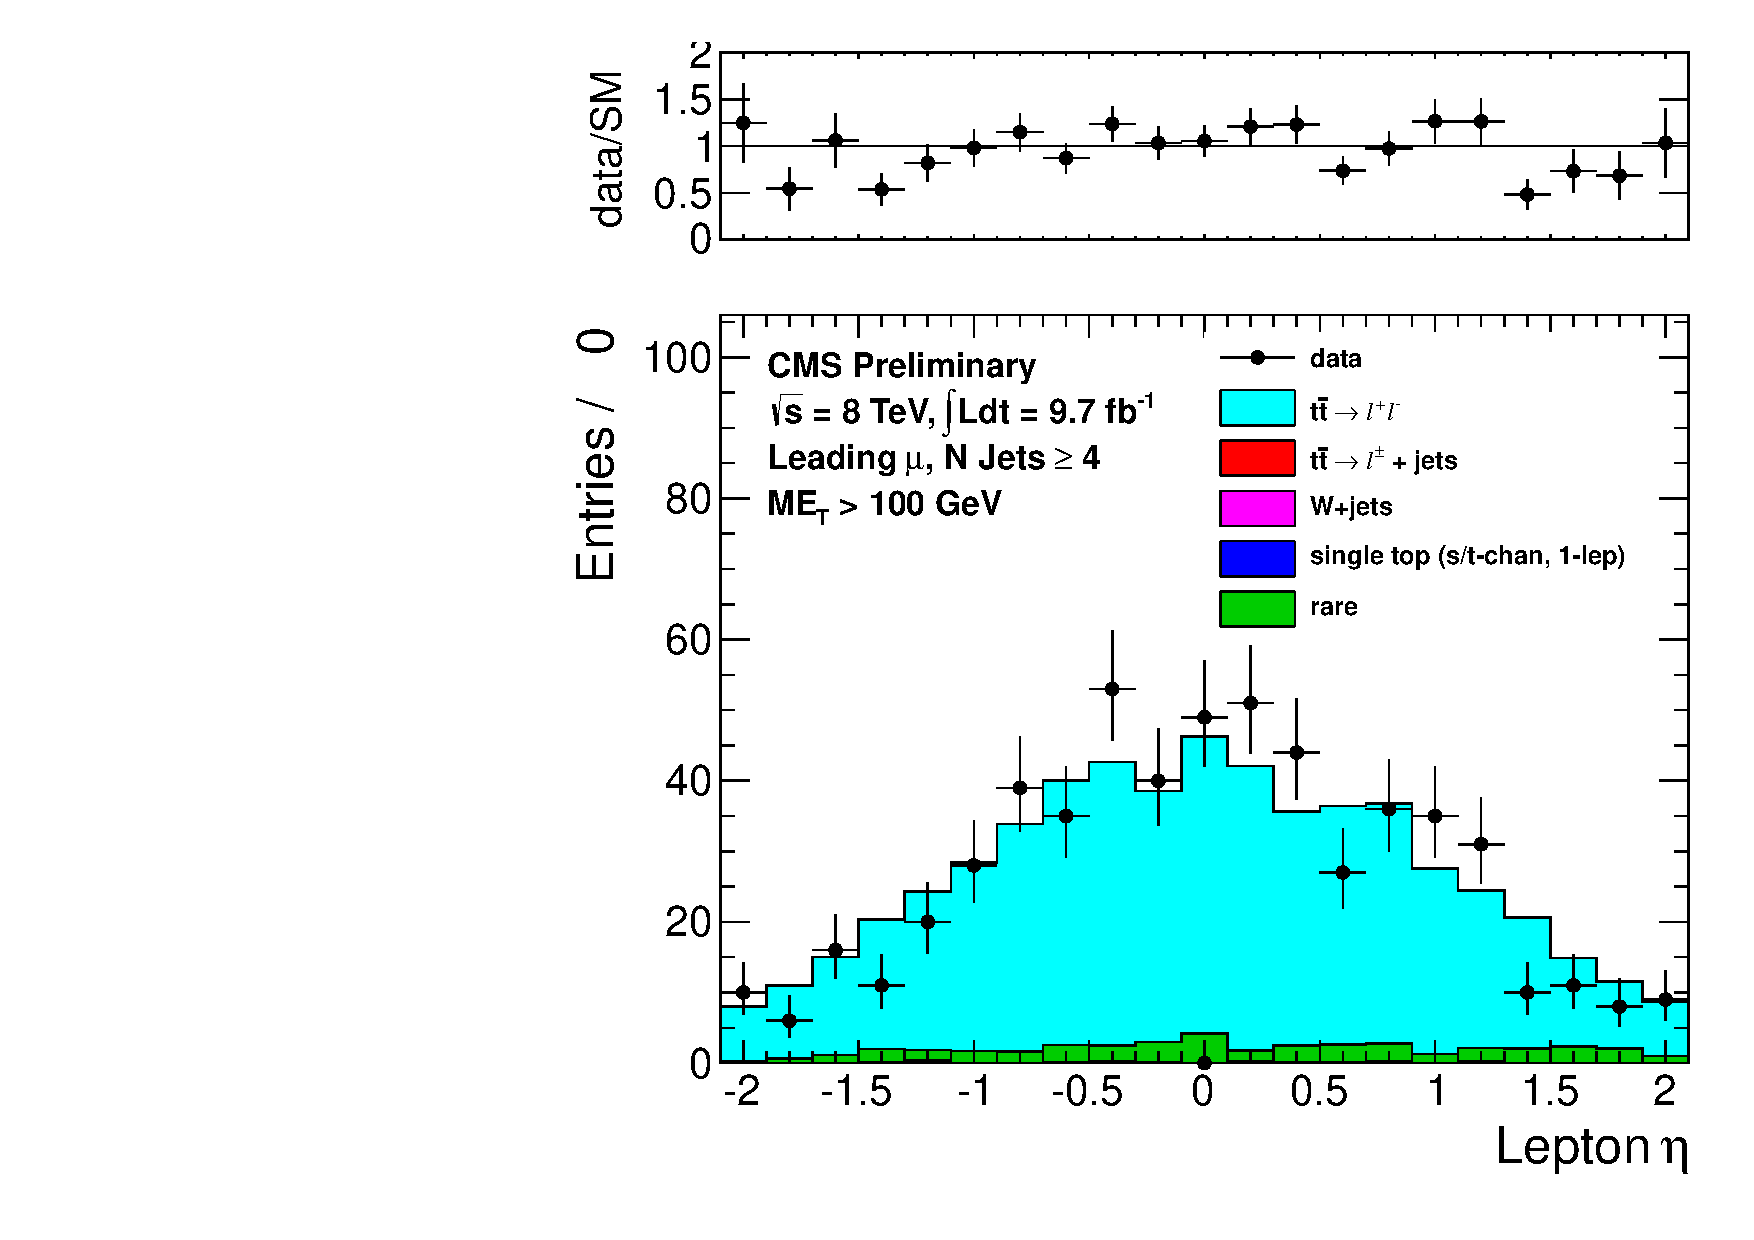
\includegraphics[width=0.5\linewidth]{plots/CR4plots/lepeta_met100_leadmuo_nj4.pdf}%
        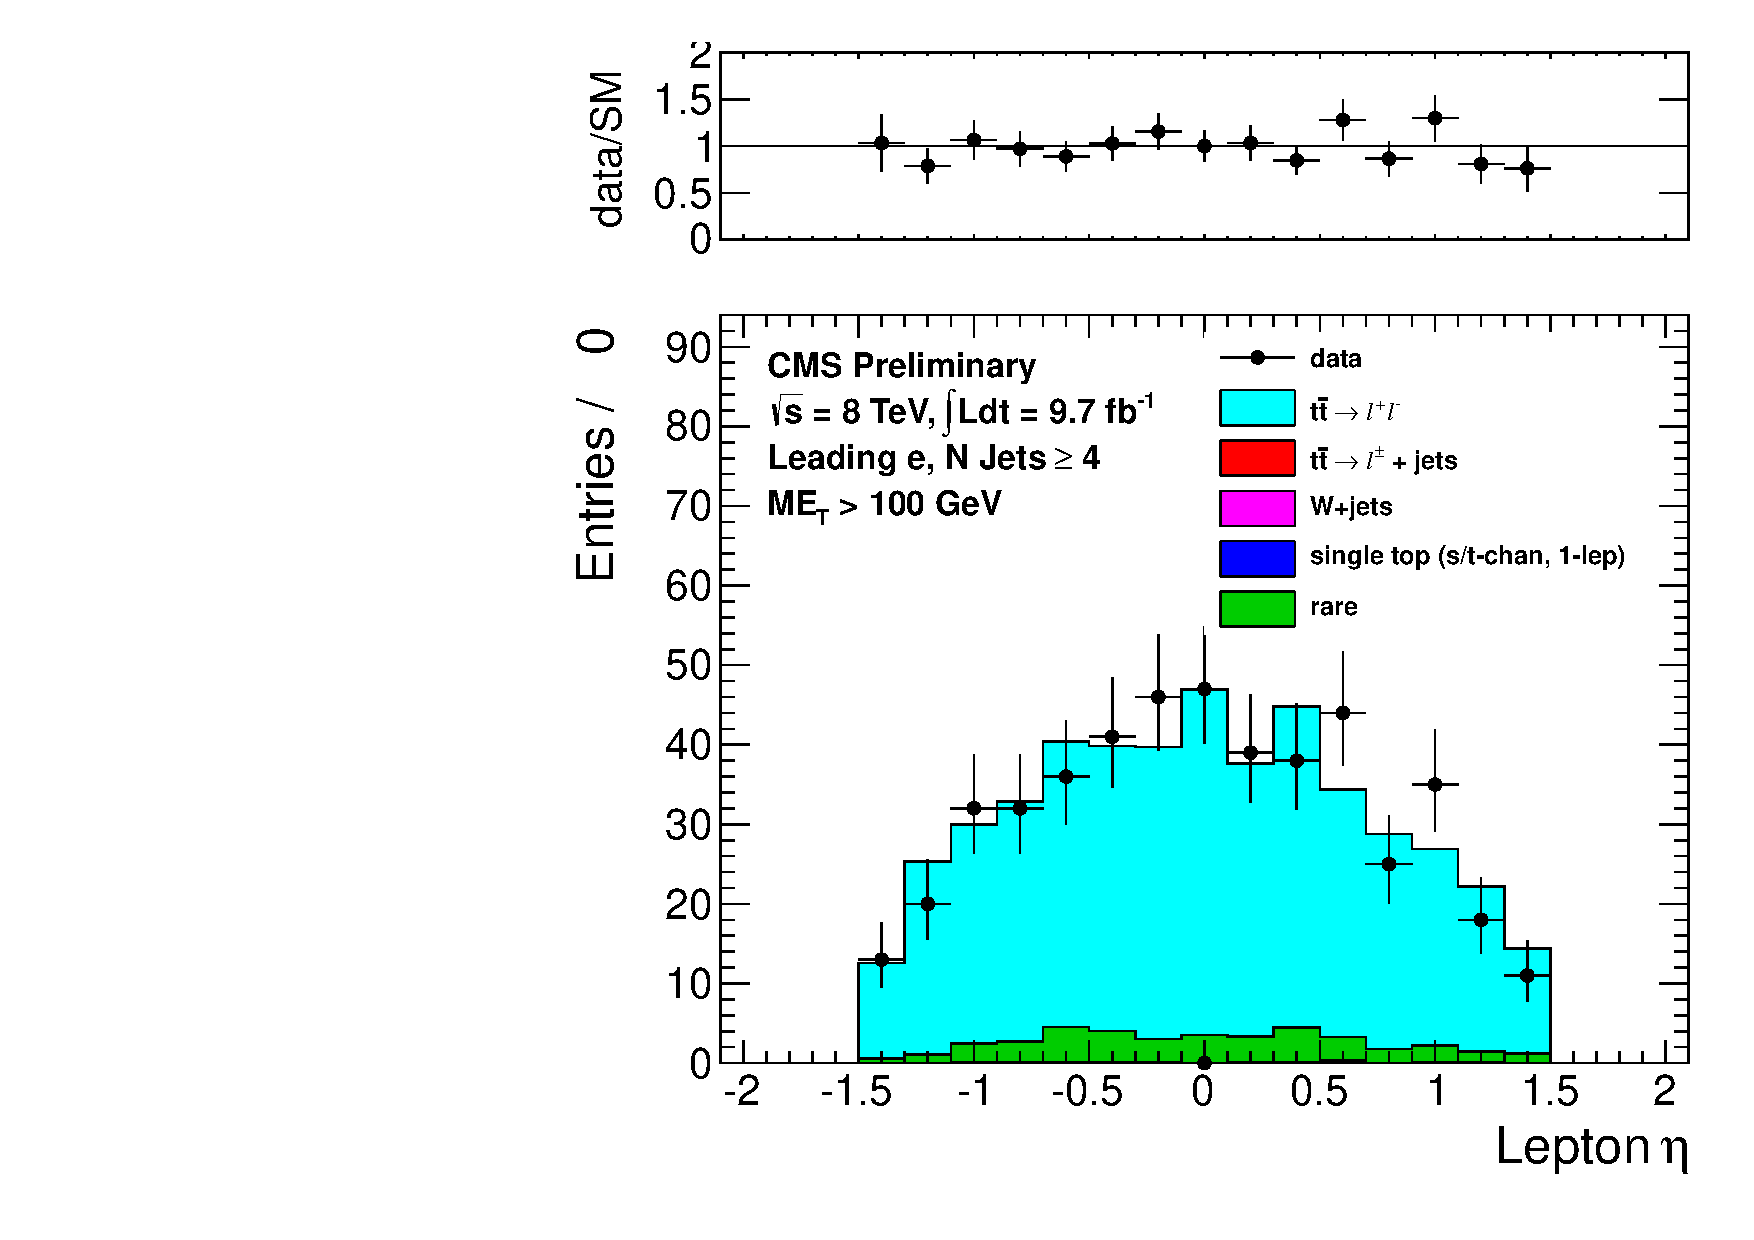
\includegraphics[width=0.5\linewidth]{plots/CR4plots/lepeta_met100_leadele_nj4.pdf}
        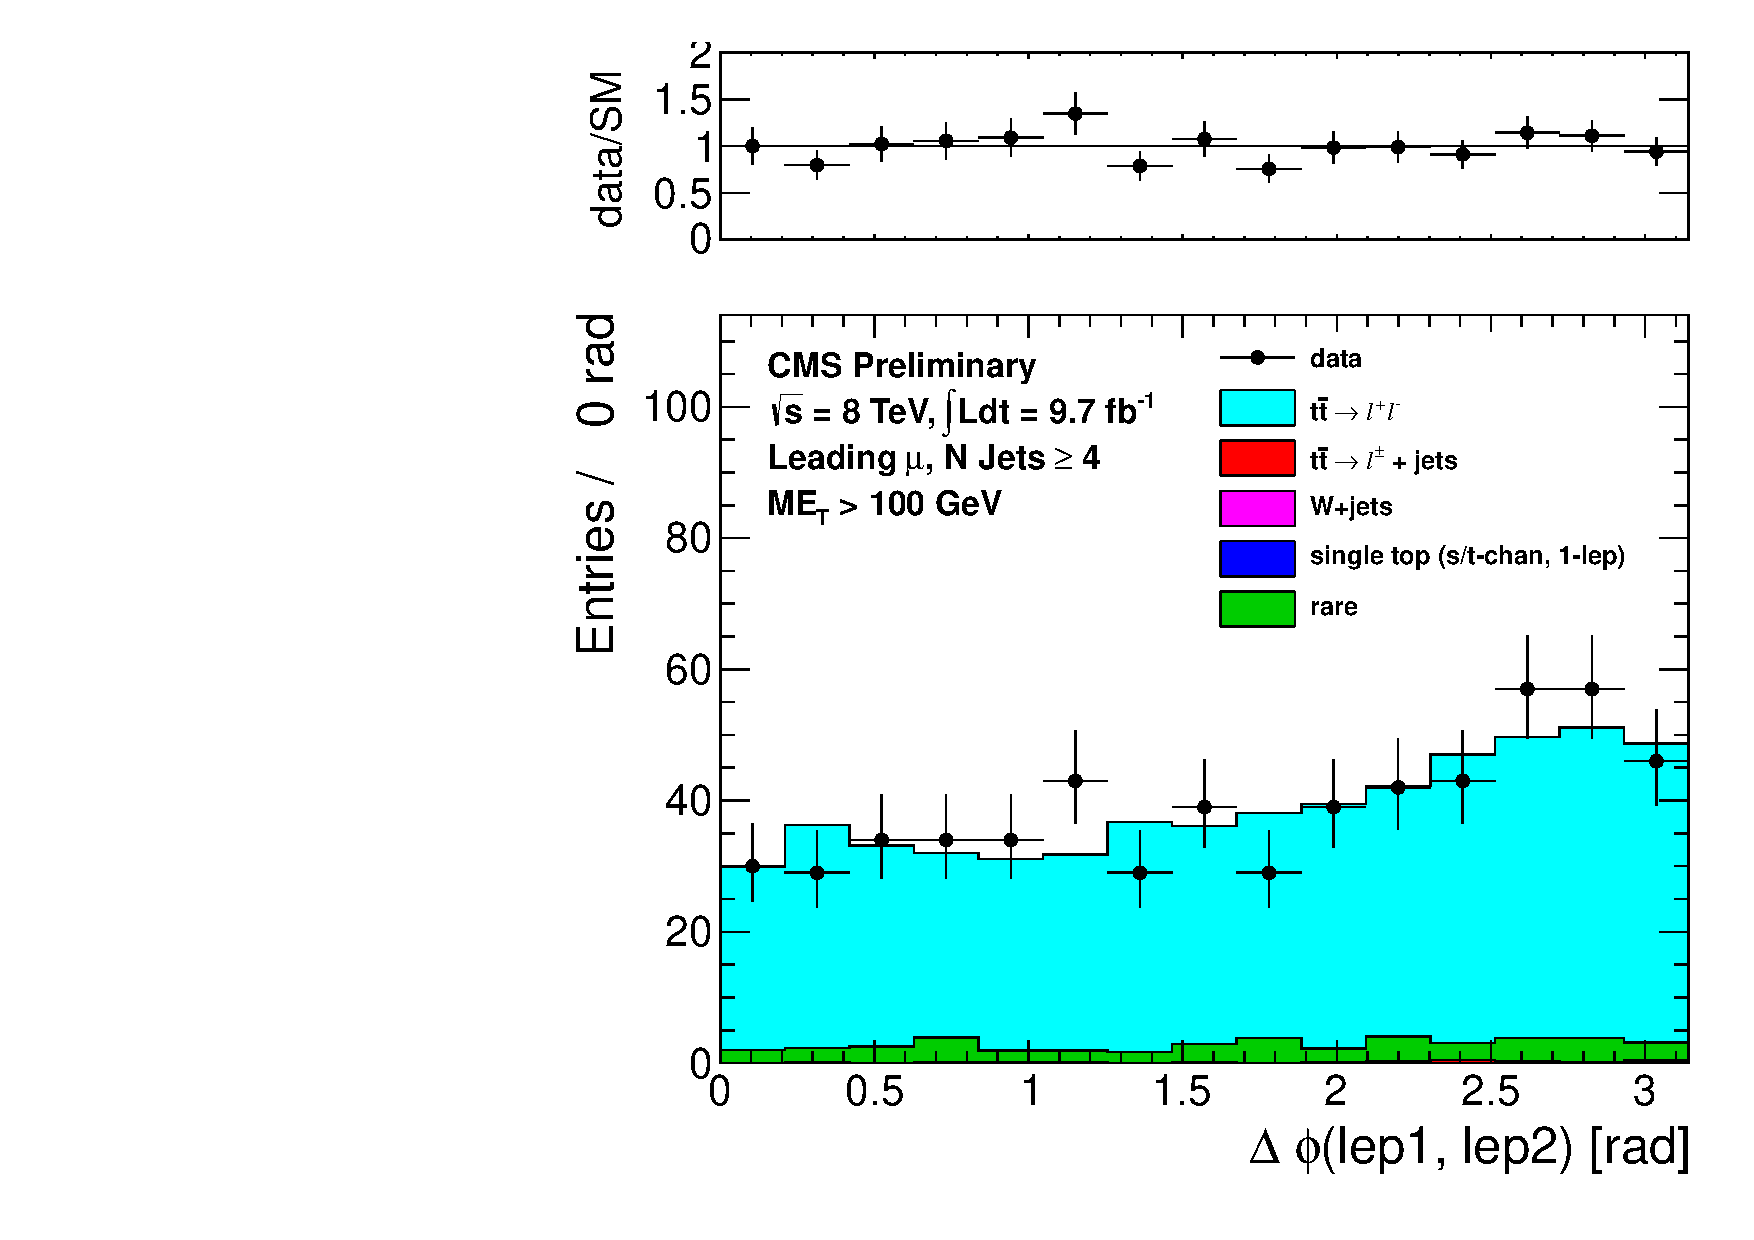
\includegraphics[width=0.5\linewidth]{plots/CR4plots/dphi_dilep_met100_leadmuo_nj4.pdf}%
        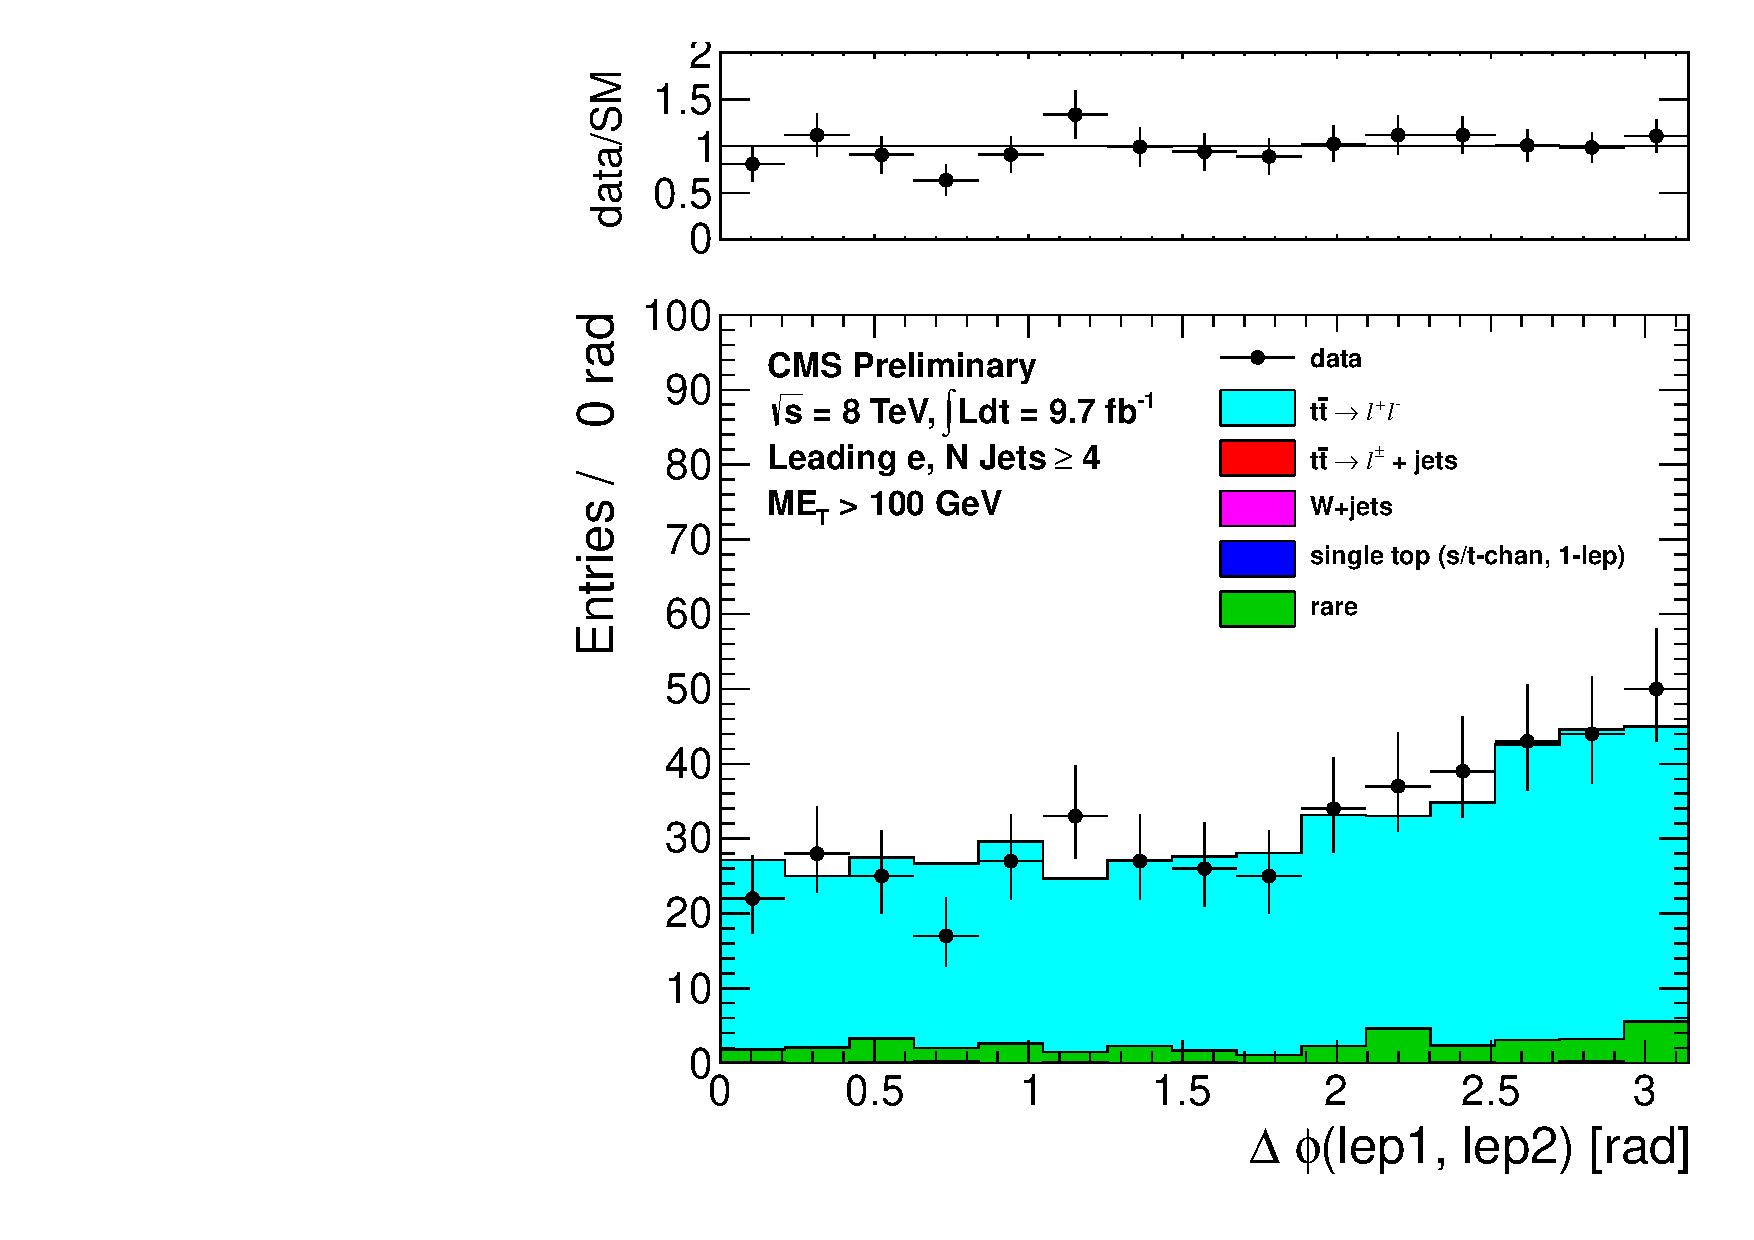
\includegraphics[width=0.5\linewidth]{plots/CR4plots/dphi_dilep_met100_leadele_nj4.pdf}
        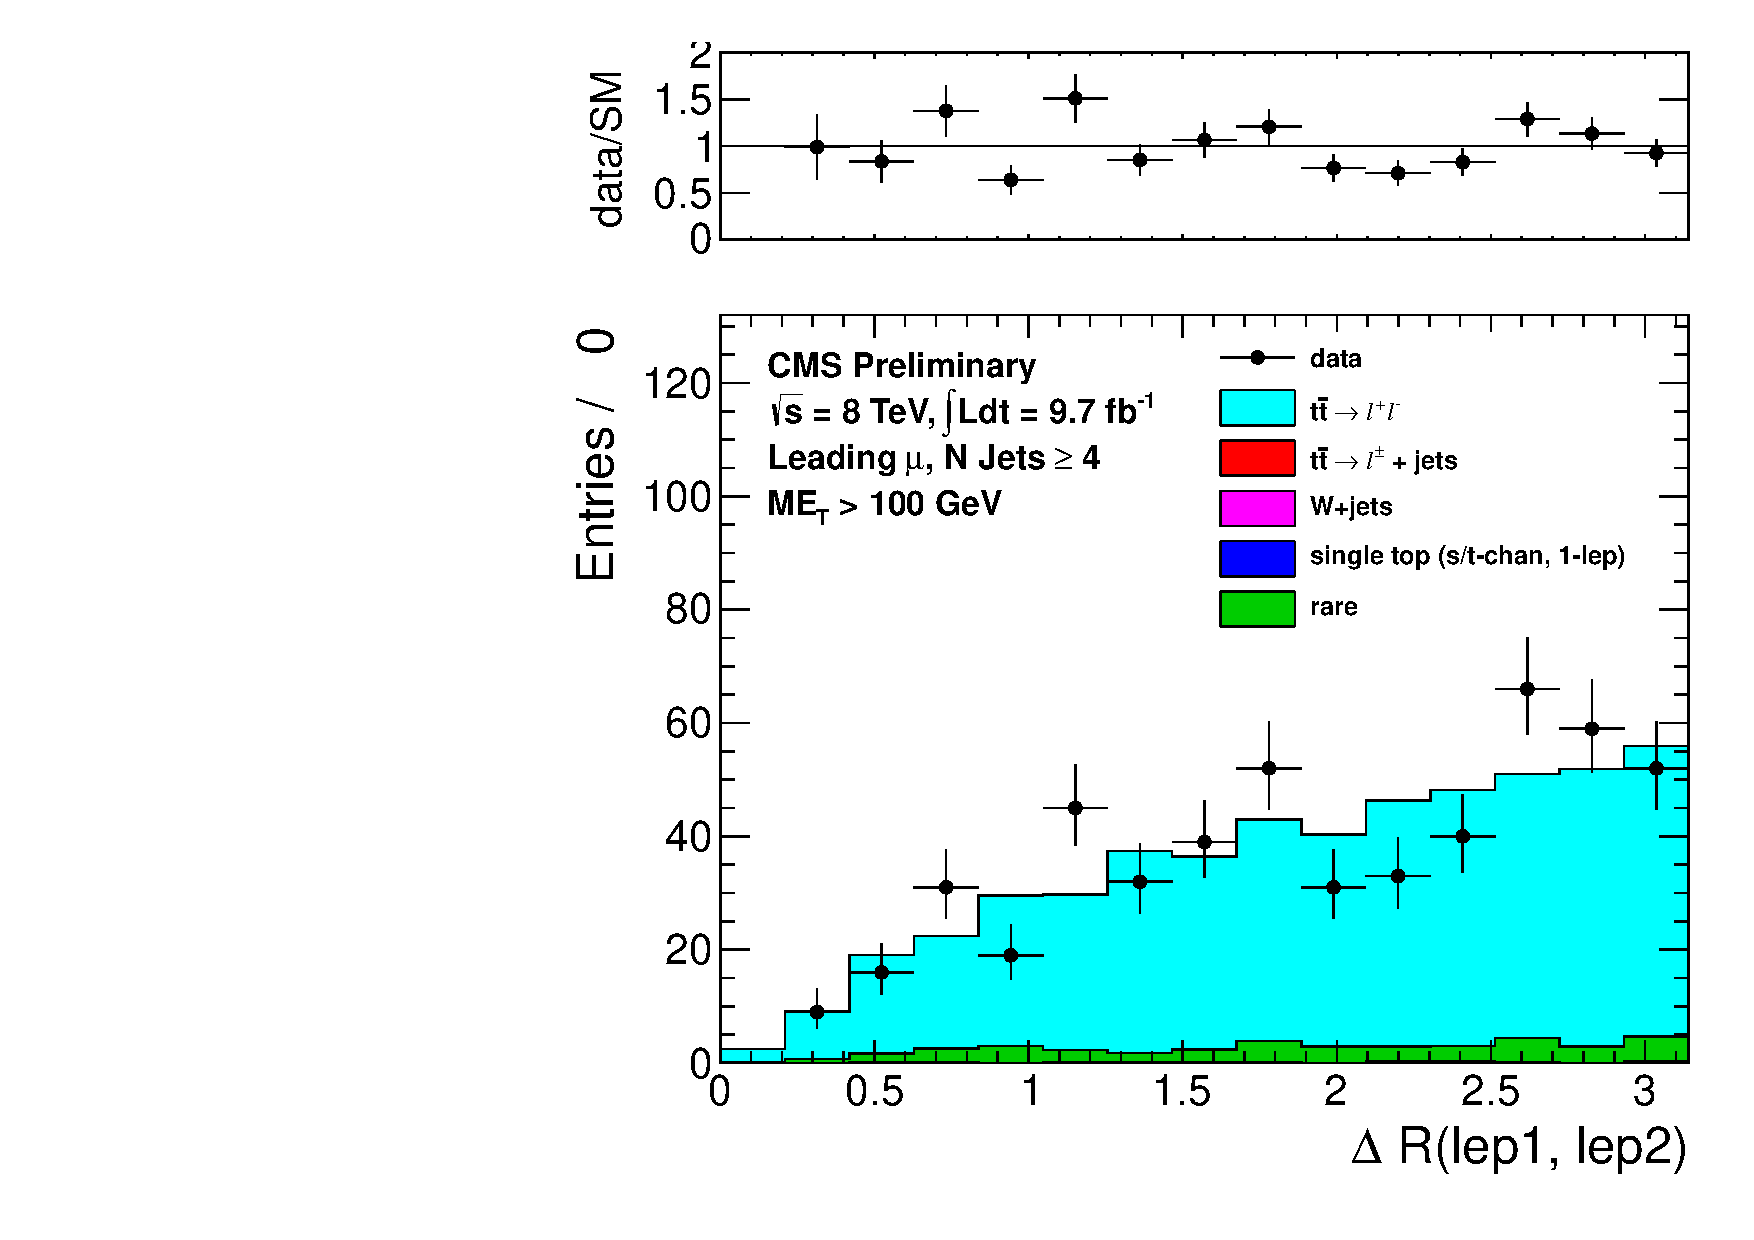
\includegraphics[width=0.5\linewidth]{plots/CR4plots/dR_dilep_met100_leadmuo_nj4.pdf}%
        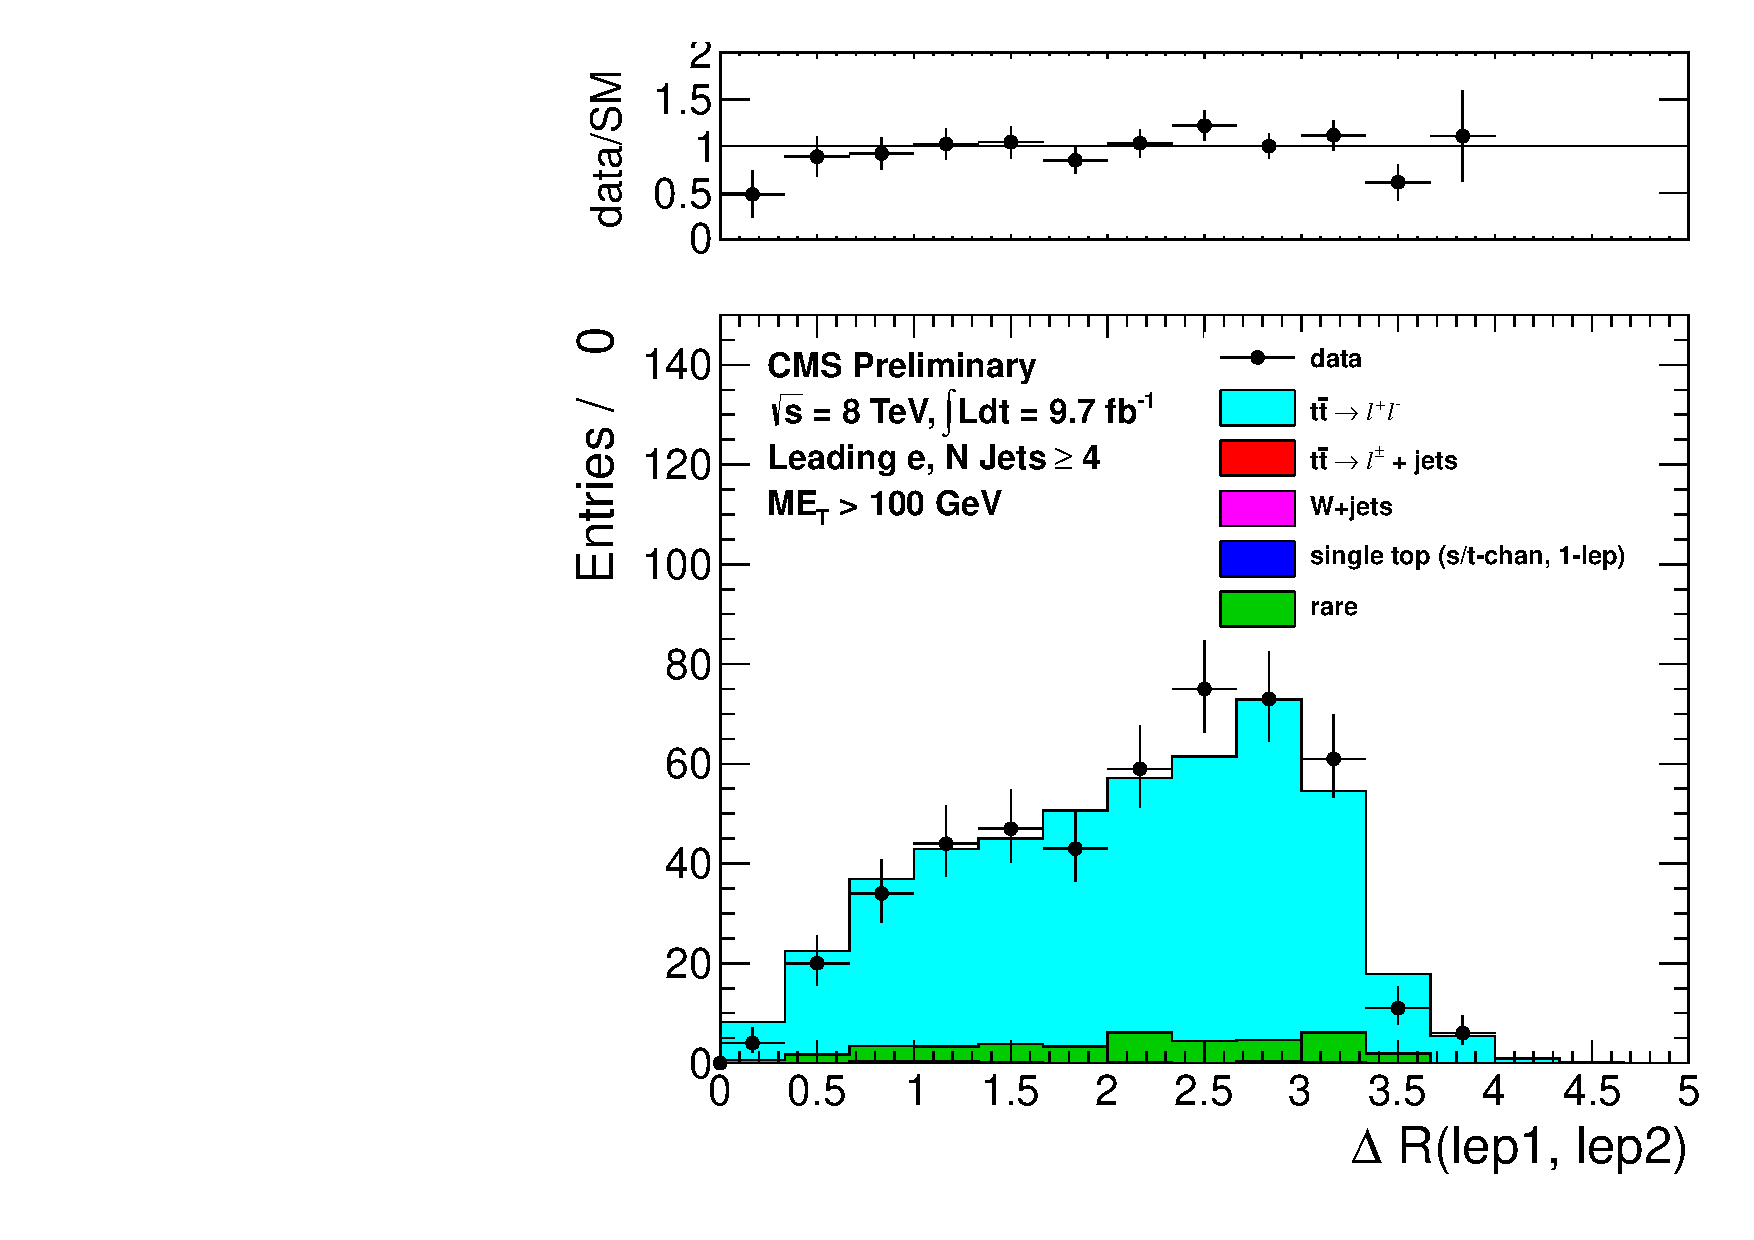
\includegraphics[width=0.5\linewidth]{plots/CR4plots/dR_dilep_met100_leadele_nj4.pdf}
    \caption{
      Comparison of the leading lepton eta (top), difference in the azimuthal 
      angle (center) and $\Delta R$ separation (bottom) between the two leptons 
      for $\met>100$ GeV distributions in data vs. MC for events
      with a leading muon (left) and leading electron (right)
      satisfying the requirements of CR4. 
\label{fig:cr4dphidR100} 
}  
      \end{center}
\end{figure}

\begin{figure}[hbt]
  \begin{center}
        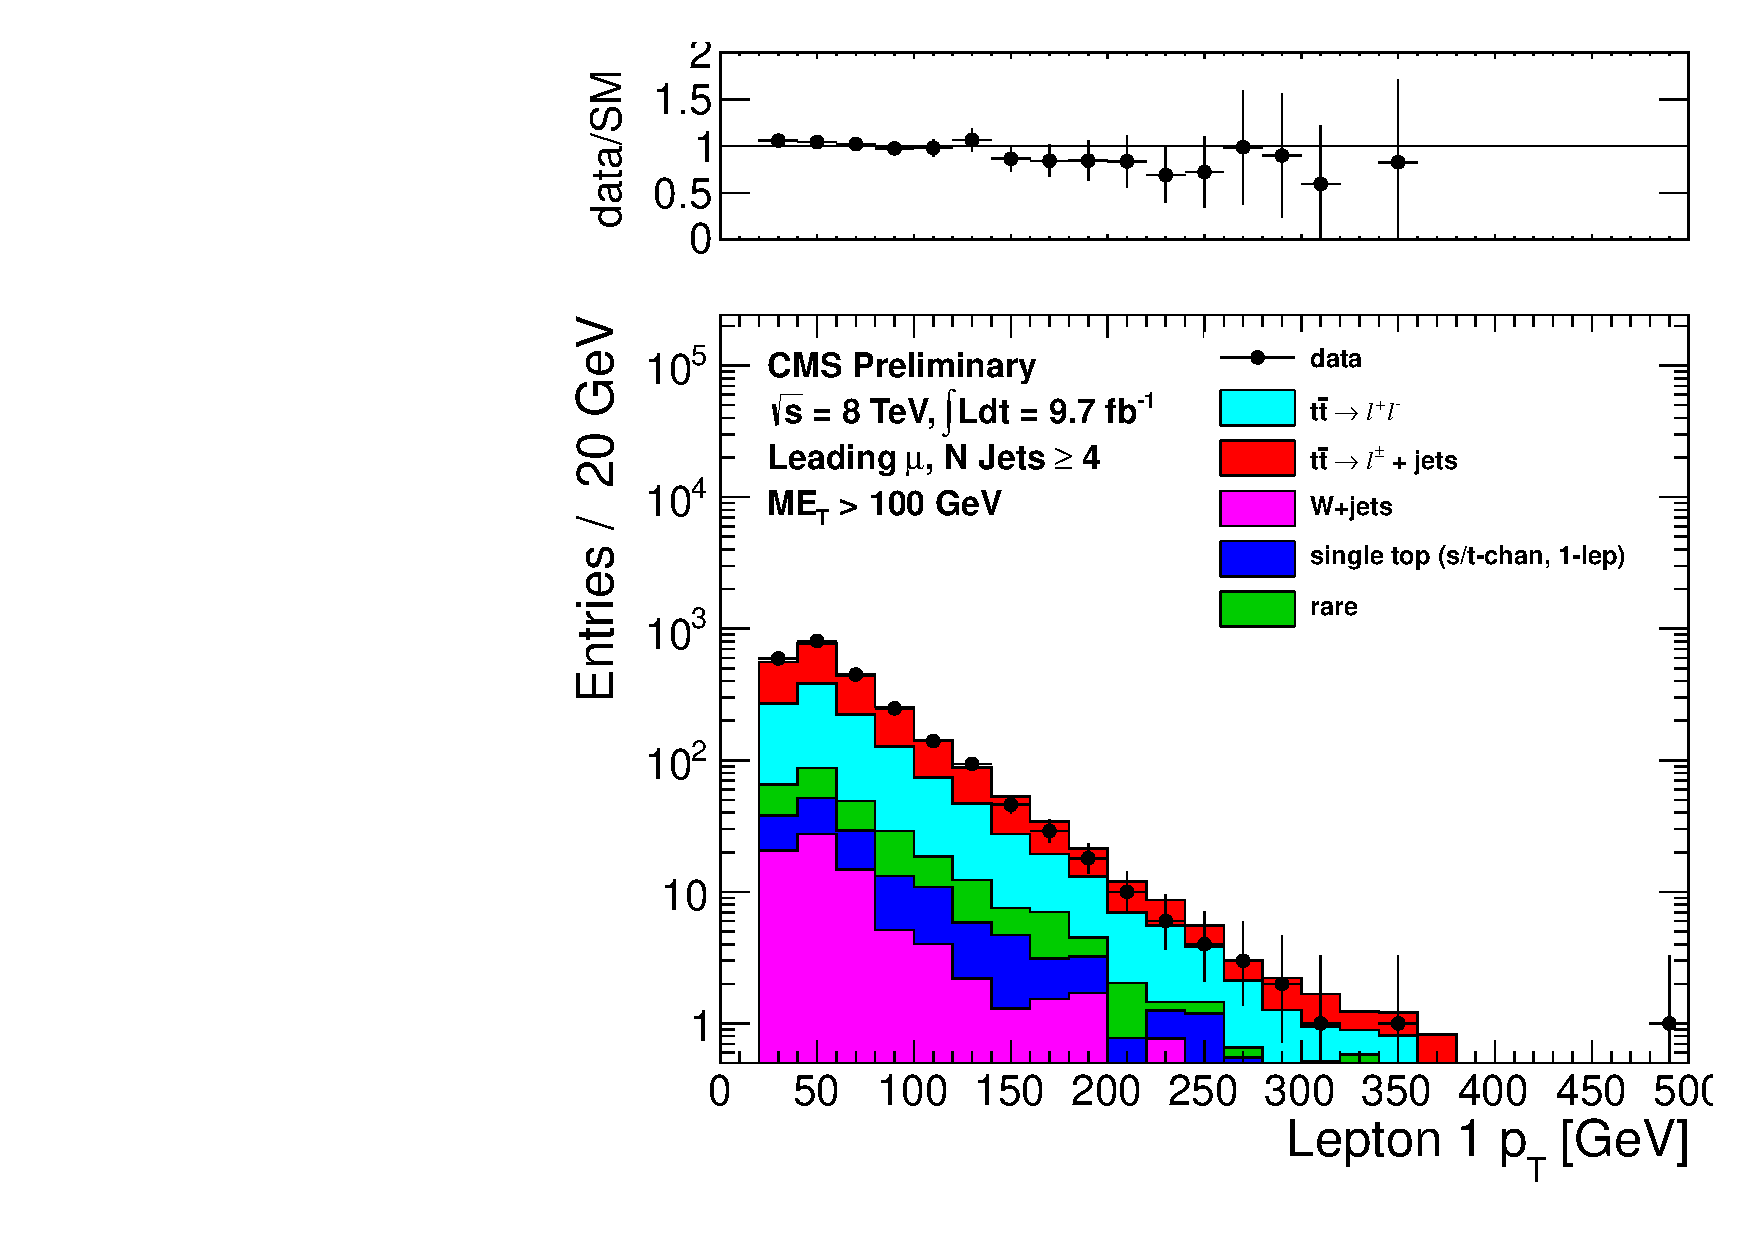
\includegraphics[width=0.5\linewidth]{plots/CR5plots/leppt_met100_leadmuo_nj4.pdf}%
        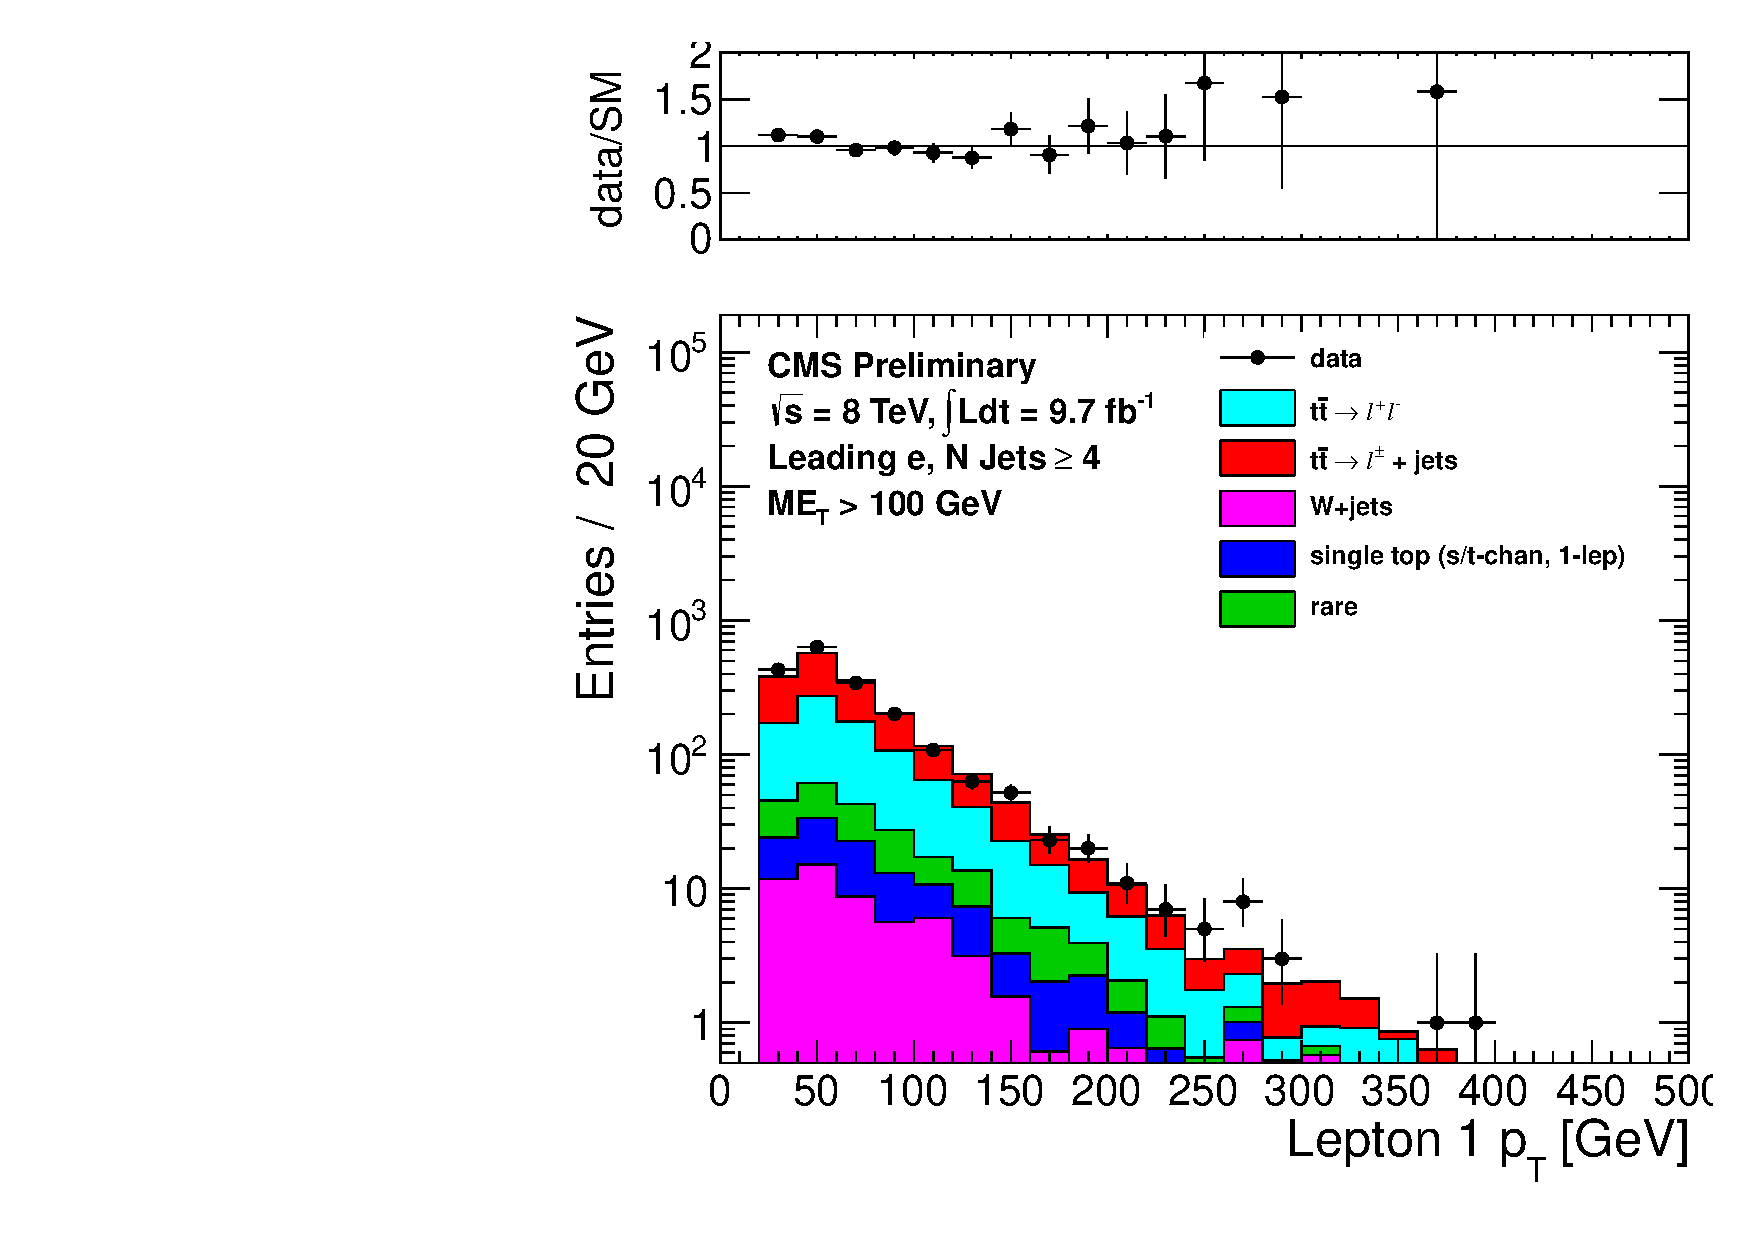
\includegraphics[width=0.5\linewidth]{plots/CR5plots/leppt_met100_leadele_nj4.pdf}
        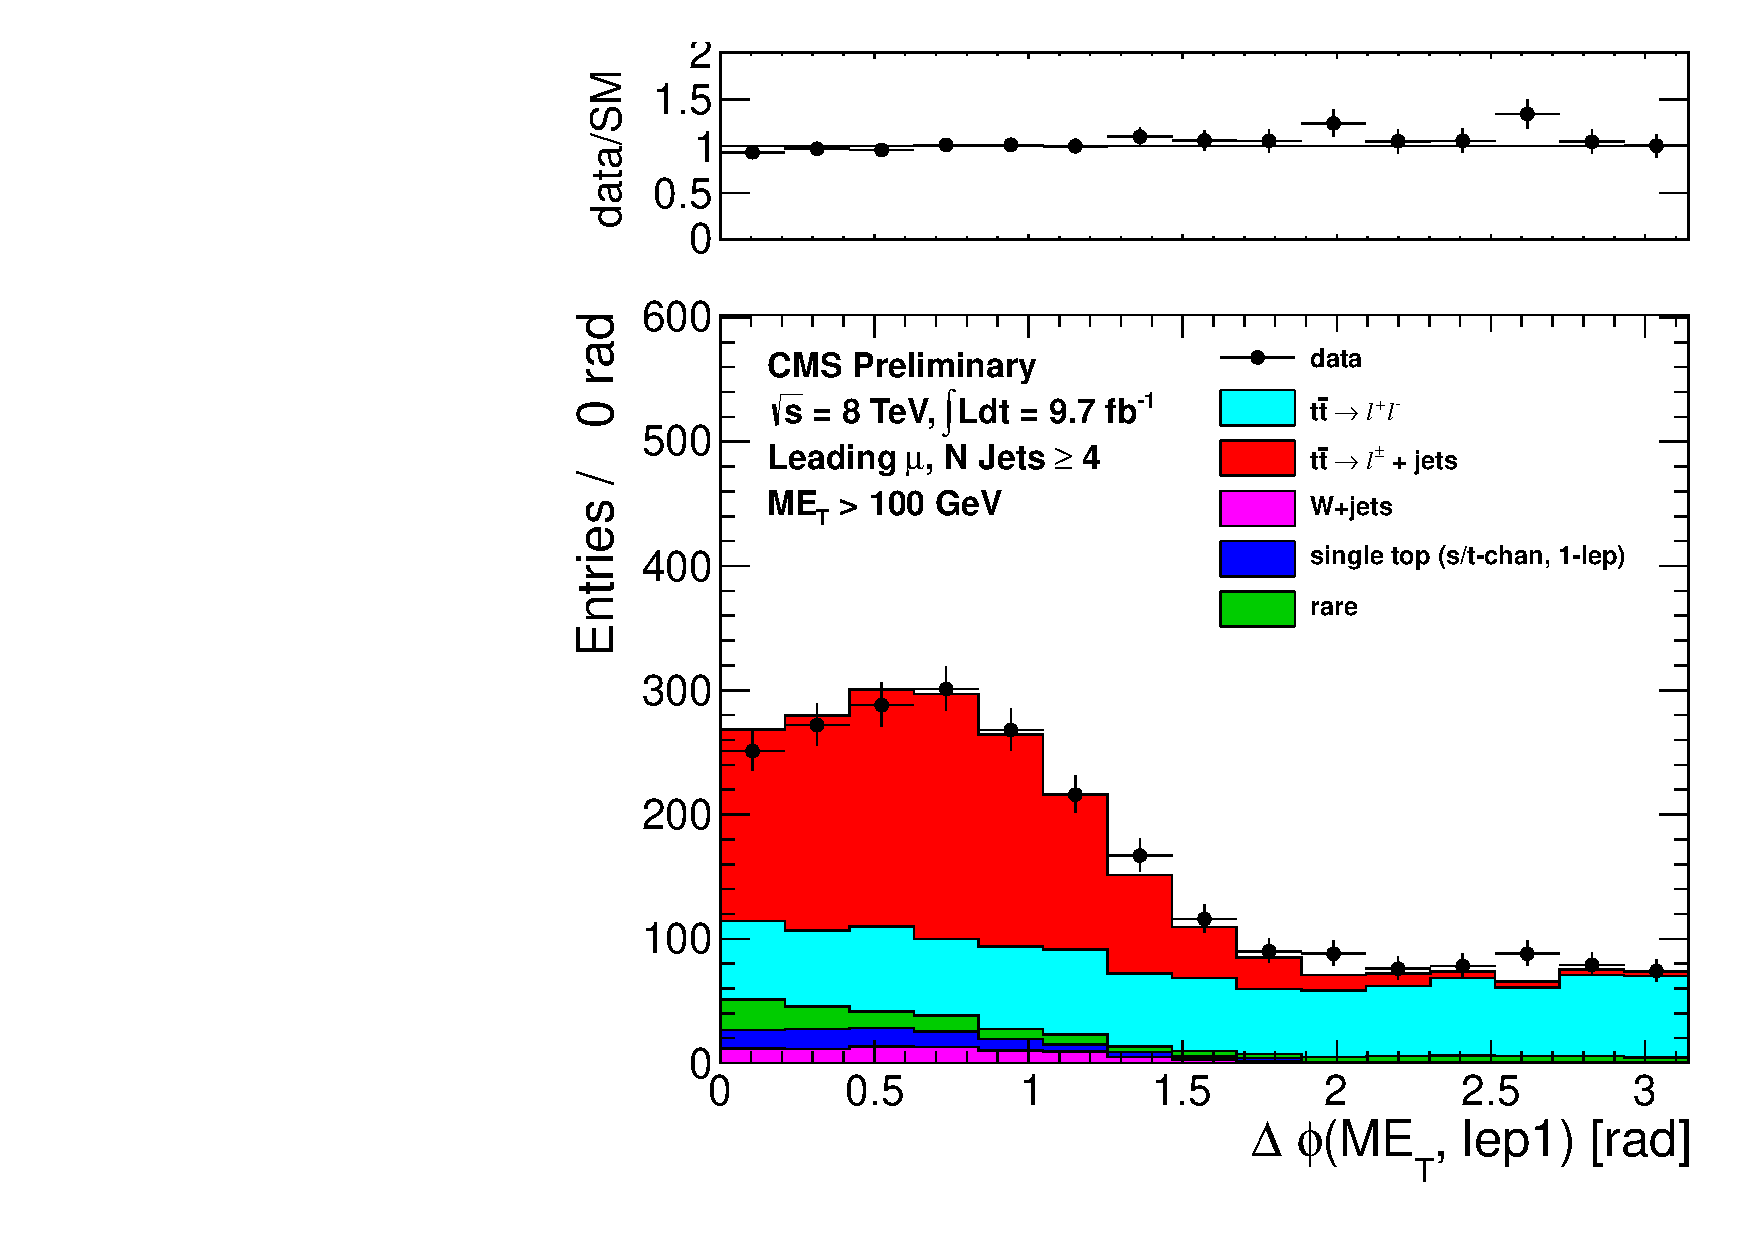
\includegraphics[width=0.5\linewidth]{plots/CR5plots/dphi_metlep_met100_leadmuo_nj4.pdf}%
        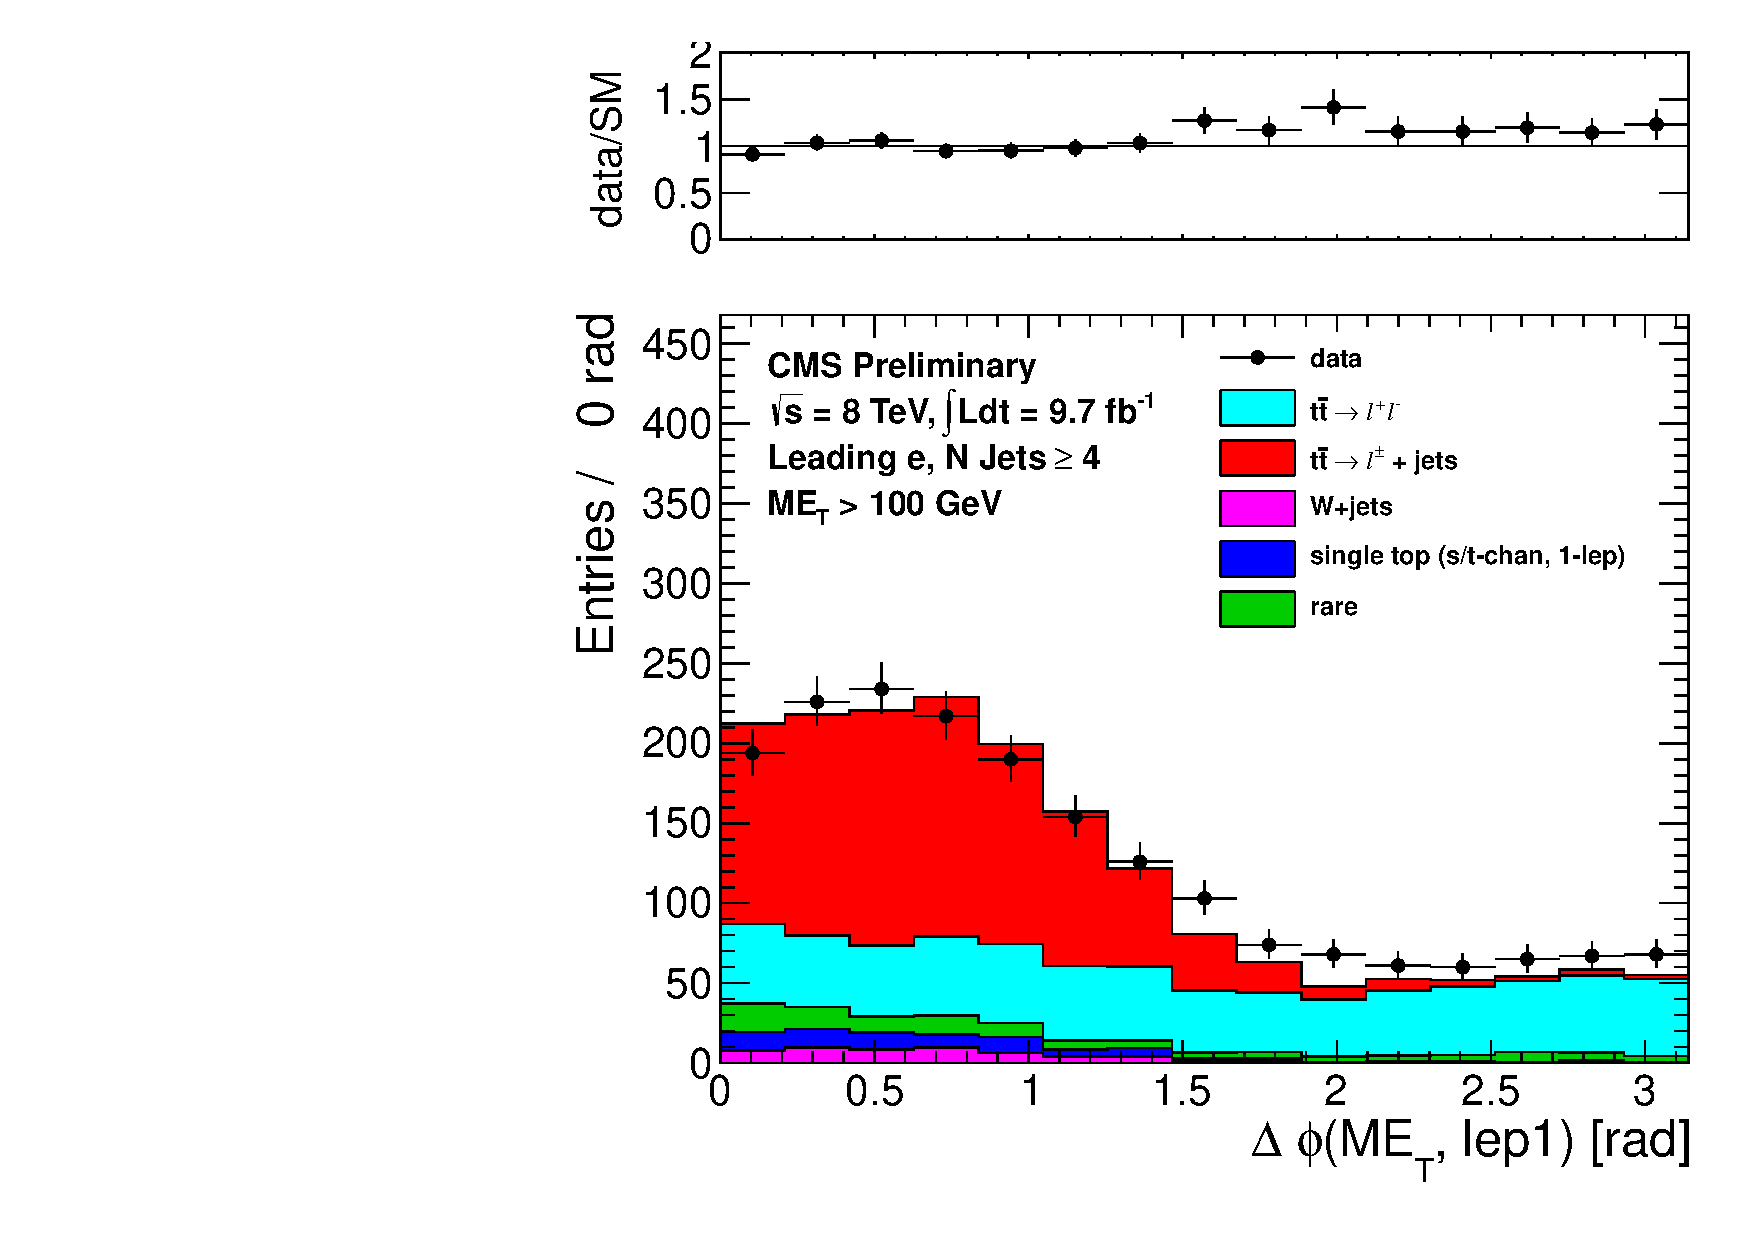
\includegraphics[width=0.5\linewidth]{plots/CR5plots/dphi_metlep_met100_leadele_nj4.pdf}
    \caption{
      Comparison of the lepton \pt\ (top) and azimuthal angle between the \met\ and the lepton (bottom) for 
      data vs. MC for $\met>100$ GeV for events with a leading muon (left) and leading electron (right)
      satisfying the requirements of CR5. 
\label{fig:cr5lepptdphi100} 
}  
      \end{center}
\end{figure}

\clearpage